\chapter[Inversion Theory: Foundations]{Inversion Theory\\ {\LARGE Foundations}}\label{ch:inversion}

\epigraph{``Reports that say that something hasn't happened are always interesting to me, because as we know, there are known knowns; there are things we know we know. We also know there are known unknowns; that is to say we know there are some things we do not know. But there are also unknown unknowns---the ones we don't know we don't know. And if one looks throughout the history of our country and other free countries, it is the latter category that tend to be the difficult ones.''}
{{\normalfont ---\ Donald Rumsfeld}}

\section{Introduction}
This quote is often treated humorously, but it captures a fundamental relationship between knowledge and information that lies at the heart of scientific inference. In geophysics, and particularly in inversion theory, we are constantly navigating between what we believe we understand about the Earth and what remains uncertain, hidden, or even unsuspected. Figure~\ref{fig:rumsfeld} provides a conceptual framework for organizing these ideas.

\begin{figure}[hbtp]
    \centering
    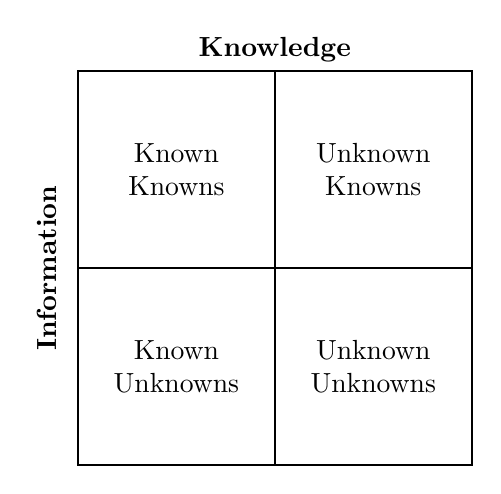
\begin{tikzpicture}[scale=1, every node/.style={align=center}]
        % Axes
        \draw[-, thick] (-2.5,0) -- (2.5,0);
        \node[rotate=90] at (-2.9, 0) {\textbf{Information}};
        \draw[-, thick] (0,-2.5) -- (0,2.5);
        \node[above] at (0, 2.5) {\textbf{Knowledge}};

        % Quadrants
        \draw[thick] (-2.5,-2.5) rectangle (2.5,2.5);

        % Labels
        \node at (-1.25,1.25) {Known\\ Knowns};
        \node at (-1.25,-1.25) {Known\\ Unknowns};
        \node at (1.25,1.25){Unknown\\ Knowns};
        \node at (1.25,-1.25){Unknown\\ Unknowns};

    \end{tikzpicture}
    \caption{Conceptual diagram, now called the Rumsfeld Matrix, can be used to describing the relationship between knowledge of a system and its properties.}
    \label{fig:rumsfeld}
\end{figure}


In its simplest form, \emph{inversion} is the process of using observations to infer properties of a system. More precisely, inversion seeks to estimate unknown properties of a system using measurements and a set of assumed physical laws**. Because observations are always incomplete and noisy, inversion is not merely a process of calculation, but one of reasoning: validating what is known, quantifying what is uncertain, and recognizing the limits of inference.

The four quadrants of Figure~\ref{fig:rumsfeld} highlight different relationships between information and knowledge:
\begin{description}
    \item[Known Knowns:]
    Characteristics of a system that we are aware of and explicitly represent. These include established physical laws, known geological processes, mapped structures, and assumptions that are consciously incorporated into models and forward operators.

    \item[Known Unknowns:]
    Aspects of the system that we recognize as uncertain. These are quantities we know exist but do not know their values, such as subsurface property distributions or interface geometries. Inversion methods are designed primarily to estimate these quantities.

    \item[Unknown Knowns:]
    Information about the system that we possess but do not yet recognize as knowledge. This information may be encoded implicitly in data structure, correlations, contextual understanding, or prior experience, but is not explicitly incorporated into the model. Much scientific progress involves recognizing and formalizing such information.

    \item[Unknown Unknowns:]
    Aspects of the system that lie outside our awareness and violate our assumptions. These include missing or incorrect physics, unrecognized processes, or fundamentally invalid model hypotheses. Persistent or systematic misfit between observations and predictions may signal the presence of unknown unknowns.
\end{description}

In this sense, inversion is not solely about estimating parameters. Progress often comes from recognizing structure in residuals, realizing constraints we already had, and promoting information from unknown knowns to known knowns or unknown unknowns to known unknowns.

Inversion theory has deep roots in geophysics. Unlike many laboratory sciences, where experiments are designed to isolate unknown physical processes, geophysics more often applies well-established physics to systems whose source distributions or material properties are unknown. We measure fields at or near the Earth's surface and seek to infer the properties and structures that produced them. This reversal---known physics applied to unknown causes---is precisely the setting in which inverse problems arise.

To illustrate the distinction between forward and inverse problems, consider the simple linear relationship
\[
    y = mx .
\]
If the values of $m$ and $x$ are known, this equation can be used to predict $y$; this is a forward problem. In reality, $y$ is measured at the conditions of $x$, but the property of the system, $m$, is unknown.  The equation can be rearranged, inverted, to solve for $m$,
\[
    m = \frac{y}{x} .
\]
This is a trivial example of an inverse problem: determining an unknown quantity from observations using a known relationship.

Most geophysical inverse problems are far more complicated. The relationships between observations and properties are often nonlinear, the number of unknowns may exceed the number of measurements, and observations are contaminated by noise. In such cases, inversion is no longer a matter of algebraic rearrangement, but requires systematic approaches to estimation, uncertainty, and interpretation. The remainder of this chapter develops the framework needed to address these challenges.

\section{Notation}

\begin{table}[h!]
    \centering
    \begin{threeparttable}
    \caption{Notation used for inverse theory in this text.}
    \label{tab:inverse_notation}
    \begin{tabularx}{0.65\textwidth}{@{}cX@{}}
        \toprule
        \textbf{Symbol} & \textbf{Quantity} \\
        \midrule
        $\vb{d}, (\vb{\tilde{d}})$    & data (pseudodata) vector \\
        $\vb{m}$    & model vector \\
        $\Fop$      & forward model/operator \\
        $\vb{J}$    & linearized sensitivity/Jacobian \\
        $\vb{A}$    & linear forward matrix\tnote{a} \\
        $\vb{C}$    & covariance \\
        $\phi$      & objective/misfit function \\
        $\vb{L}$    & regularization operator \\
        $\vb{r}$    & residual \\
        $\vb{W}$    & weighting matrix \\
        $\epsilon$  & noise/error \\
        $\lambda$   & Lagrangian multiplier/regularization hyperparmeter\tnote{b} \\
        $\Delta$    & small perturbation (step) \\
        \bottomrule
    \end{tabularx}
    \begin{tablenotes}
    \item[a] While we use $\vb{A}$ in this text, $\vb{G}$ is probably more common in geophysics.  We use $\vb{A}$ so it is not confused with the gravitational constant.
    \item[b] Hyperparameters are external (non-physical) variables that are used to tune a the behavior/performance of the inversion.  These are either set manually by the user or optimized by a grid search or some other process. They affect the complexity and accuracy of an inversion.
    \end{tablenotes}
    \end{threeparttable}
\end{table}


\section{Inversion and Curve-Fitting}

At its core, inversion is a problem of estimation. Observations are related to a set of parameters through a mathematical model, and the objective of inversion is to determine the parameter values that best explain the data. In this sense, geophysical inversion is not fundamentally different from curve fitting or regression: both seek to infer unknown quantities from measurements using an assumed functional relationship.

This perspective is useful because it emphasizes that inversion methods are not uniquely tied to geophysics. The same mathematical framework can be applied to a wide variety of problems, including fitting experimental data in the laboratory, calibrating analytic models, analyzing synthetic data, or interpreting field observations. What distinguishes geophysical inversion is not the mathematics itself, but the physical meaning ascribed to the parameters and the interpretation of the resulting models.

Historically, inversion techniques have emerged independently in multiple disciplines, often under different names and with different terminology (Box~\ref{box:inverse_terms}). In statistics, similar problems are referred to as estimation or regression; in data science and machine learning, they are described in terms of training models or fitting predictors. Despite these differences in language, the underlying ideas are closely related. Recognizing these connections can help demystify inversion methods and place them within a broader scientific context.

From the curve-fitting viewpoint, inversion can be seen as the task of finding the model that minimizes the discrepancy between observed data and predictions generated by a forward relationship. The forward relationship encodes prior knowledge in the form of physical laws or empirical models, while the observed data provide constraints. In practice, this discrepancy cannot usually be reduced to zero, because measurements are noisy, models are imperfect, and the parameterization is necessarily incomplete. As a result, inversion becomes a problem of compromise: determining which models are consistent with the data to an acceptable degree.

This framing also highlights an important conceptual shift. Rather than asking whether a single model is correct, inversion asks which models are compatible with both the observations and the assumptions imposed by the forward model. The goal is not simply to compute parameter values, but to understand how information contained in the data constrains the model, what remains uncertain, and how sensitive the conclusions are to the underlying assumptions.

The sections that follow develop this idea in progressively more detail, beginning with linear inverse problems and least-squares estimation, and later addressing uncertainty, nonuniqueness, regularization, and nonlinear inversion. Throughout, it is useful to keep in mind that these techniques are general tools for estimation, adapted to the specific challenges posed by geophysical data.

\ntextbox{Comparative Terminology}{
    The concepts of inversion theory have been used in many scientific and mathematics fields, sometimes independently.  This independence has resulted in differences in terminology.  So if these concepts feel familiar but you don't understand the jargon, it may be because you have seen/used these before in a different context.  While the terms below aren't fully developed until later in this chapter, a rough translation is given in the table below (Table~\ref{tab:inverse_terms}).
    \begin{center}
        \textbf{Table~\thetable:} Inversion theory terminology varies between fields.
        \label{tab:inverse_terms}
        \begin{tabularx}{\textwidth}{cXXXX}
        \toprule
        & Geophysics & Physics & Statistics & Machine Learning \\
        \midrule

        {} 
        & inversion theory 
        & parameter estimation 
        & regression / inference 
        & training \\

        {} 
        & inverse problem 
        & fitting / inverse problem 
        & statistical inference 
        & optimization \\

        {} 
        & least-squares inversion 
        & least-squares estimation 
        & linear regression 
        & least-squares training \\

        $\Fop$ 
        & forward operator 
        & forward model 
        & model (linear case: design matrix) 
        & model \\

        $\lambda \phi_m$ 
        & regularization 
        & prior constraint 
        & penalty term 
        & regularization \\

        {} 
        & damping 
        & stabilizer 
        & ridge penalty 
        & $L_2$ regularization \\

        $\vb{m}$ 
        & model parameters 
        & fitted parameters 
        & regression coefficients 
        & weights \\

        $\vb{r}$ 
        & residual / misfit 
        & residual 
        & error (residual) 
        & prediction error \\

        $\Phi,\ \phi$ 
        & objective (misfit) function
        & misfit function
        & negative log-likelihood / cost function 
        & loss function \\

        $\vb{C}$ 
        & model covariance 
        & parameter covariance 
        & posterior covariance 
        & uncertainty estimate \\

        {} 
        & sensitivity kernel 
        & response function 
        & explanatory variables (features) 
        & features \\

        $\vb{A}$ 
        & forward operator (linear) 
        & response matrix (linear) 
        & design matrix 
        & model matrix \\

        $\vb{J}$ 
        & Jacobian / sensitivity matrix 
        & response function (nonlinear) 
        & gradient of model prediction 
        & Jacobian / gradient \\
        \bottomrule
        \end{tabularx}
    \end{center}
}{aside}\label{box:inverse_terms}

\section{Forward Operators}

The relationship between observations and models in inversion is defined through the \emph{forward problem}. A forward problem uses an assumed set of physical laws to predict observable quantities from a specified description of the system. In the context of inversion theory, this relationship is written abstractly as
\begin{equation}
    \coreeq
    \mlbox[
        labelstyle={xshift=-1cm},
        linestyle={out=270,in=90, latex-}]
        {\Fop}{physics}
    \mlbox[
        labelstyle={below of=m\themathLableNode,below of=m\themathLableNode}]
        {(\vb{m})}{physical properties}
    = \mlbox[]{\tilde{\vb{d}}}{fields} ,
    \label{eq:foward}
\end{equation}
where $\vb{m}$ represents the model parameters, $\tilde{\vb{d}}$ represents the predicted data, and $\Fop$ is the \emph{forward operator}.  While the equation above hides much of the complexities involved in the forward solution, it captures the similarity of the process that we can follow for nearly all of our geophysical inverse problems.  The forward operator encapsulates the governing physics, geometry, boundary conditions, and measurement configuration relevant to the problem.

This notation emphasizes that inversion does not invent new physics. Instead, it relies entirely on the forward operator to connect models to data. Every inverse problem is therefore constrained, limited, and shaped by the assumptions embedded in $\Fop$. This operator contains the `rules' of the system under investigation, telling us how changes in Earth's physical properties and source geometry affect the strength of the fields that we measure.  The physical properties of Earth (the model parameters) are contained within $m$ and the observed fields (data) are denoted by $d$.  A list of the $d$ and $m$ are given for several geophysical processes in Table~\ref{tab:invar}.
\begin{table}[hbt]
    \centering
    \caption{Examples of geophysical inverse problems showing the relationship between observed data and model parameters.}
    \label{tab:invar}
    \begin{tabular}{@{}lll@{}}
        \toprule
        Physical process & Data (observed) & Model (inferred) \\
        \midrule
        gravitation & gravity field & density \\
        magnetics & magnetic field & magnetic susceptibility \\
        steady-state heat flow & temperature or heat flux & thermal conductivity, heat production \\
        thermal diffusion & temperature (time dependent) & thermal diffusivity \\
        chemical diffusion & concentration & diffusion coefficient \\
        time-domain EM & voltage or EM response & resistivity (or conductivity) \\
        frequency-domain EM & impedance & resistivity (or conductivity) \\
        seismic travel-time & travel times & seismic velocity (or slowness) \\
        seismic waveform & ground motion & velocity structure, source parameters \\
        \bottomrule
    \end{tabular}
\end{table}

It is useful to distinguish between \emph{model space} and \emph{data space}. Model space consists of all possible parameter values used to describe the Earth or system of interest, such as density, velocity, conductivity, or layer thicknesses. Data space consists of observable quantities, such as gravity anomalies, travel times, electric fields, or magnetic intensities. The forward operator defines a mapping from model space to data space, projecting abstract physical properties into measurable signals.

In principle, Earth properties vary continuously in space and time, leading to continuous models and continuous fields. In practice, both models and data must be discretized. The model is represented by a finite set of parameters, and the data by a finite collection of measurements. Discretization is not merely a computational convenience; it is a modeling choice that determines what structures can be represented and what information can be resolved. The number, meaning, and spatial distribution of model parameters are therefore central components of any inversion.

An important consequence of this formulation is that inversion inherits all limitations of the forward problem. If the forward operator is insensitive to certain aspects of the model, those aspects cannot be recovered through inversion. If important physics is omitted, the inversion may produce models that fit the data but are physically misleading. Inversion cannot compensate for incorrect assumptions or missing information; it can only work within the space of models that the forward operator allows.

Before an inverse problem is formulated, several fundamental choices must be made.  These choices define the space of admissible models and determine what information can and cannot be recovered from the data.
\begin{itemize}
    \item \textbf{Governing physics:}
    The physical laws and approximations used to relate material properties to observations (e.g., Newtonian gravity, ray theory, quasi-static electromagnetics).  This choice determines which processes are represented and which are excluded.

    \item \textbf{Parameterization:}
    determines what can vary (e.g., blocks, layers, interfaces, basis functions, contrasts) and how these unknown properties are represented mathematically. Parameterization controls linearity, resolution, and trade-offs between parameters. We'll come back to this later, but the number of parameters directly affects whether the problem is over- or under-determined.

    \item \textbf{Geometry and dimensionality:}
    determines where those parameter variations influence the data.
    The spatial domain, coordinate system, and effective dimensionality of the model (e.g., 1-, 2-, or 3-D; bounded or infinite domains; known or unknown interfaces).  These choices constrain the forms of structure that can be resolved.
\end{itemize}

These decisions define the structure of model space and determine how models are mapped into data space. Different choices can lead to very different inverse problems, even when applied to the same set of observations.

\ntextbox{Geometry influences sensitivity: Gravity of a Buried Mass}{
Consider a gravity measurement made at the Earth's surface. The vertical component of gravitational acceleration produced by a point mass mmm at depth $z$ directly beneath the measurement point can be written schematically as
\[
    g(z) \propto \frac{m}{z^2}.
\]
The exact form is not important here; what matters is the dependence on depth.  Now ask a simple sensitivity question:

\emph{How does a small change in mass at depth affect the observed gravity?}

The sensitivity of the data to the mass is proportional to
\[
    \pdv{g}{m} \propto \frac{1}{z^2}
\]
This expression shows that sensitivity decreases rapidly with depth. A change in mass at shallow depth produces a much larger change in observed gravity than the same change in mass at greater depth.  This geometric effect occurs even though the governing physics—Newton's law of gravitation—is linear in mass. This uneven sensitivity is inherent to the problem. No inversion method can amplify information that is not present in the data.
}{core}

\section{Linearity}\label{sec:linearity}

The distinction between linear and nonlinear problems plays a central role in inversion theory, just as it does in forward modelling and superposition (Section~\ref{sec:superposition}). Because many inversion methodologies rely on linear structure, it is important to be precise about what is meant by linearity and where it applies.

A mapping is said to be \emph{linear} if it satisfies two conditions: additivity and homogeneity.  Formally, if $\Fop$ denotes a forward operator and $\mathbf{m}_1$ and $\mathbf{m}_2$ are models, then linearity requires
\begin{align}
    \Fop(\mathbf{m}_1 + \mathbf{m}_2) &= \Fop(\mathbf{m}_1) + \Fop(\mathbf{m}_2), \\
    \Fop(a\,\mathbf{m}) &= a\,\Fop(\mathbf{m}),
\end{align}
for any scalar $a$. If either condition fails, the operator is nonlinear. An example of the principles is given in Box~\ref{box:linearity}.

\ntextbox{Linearity example}{
    Linearity can be illustrated using the simple straight-line relationship
    \[
        y = m x + b .
    \]
    Consider this equation as a forward model in which the independent variable $x$ is known and the parameters are $m$ and $b$. Written in operator form, the mapping from model parameters to data values can be expressed as
    \[
        y = \Fop(m,b) = m x + b .
    \]

    To test additivity, let $(m_1,b_1)$ and $(m_2,b_2)$ be two parameter sets. Then
    \begin{align*}
        \Fop(m_1+m_2,\, b_1+b_2) &= (m_1+m_2)x + (b_1+b_2) \\
        &= (m_1 x + b_1) + (m_2 x + b_2) \\
        & = \Fop(m_1,b_1) + \Fop(m_2,b_2),
    \end{align*}
    so the additivity condition is satisfied. Similarly, for any scalar $a$,
    \begin{align*}
        \Fop(a m,\, a b) &= a m x + a b \\
        &= a (m x + b) \\
        &= a\,\Fop(m,b),
    \end{align*}
    demonstrating homogeneity. The forward problem is therefore linear with respect to the parameters $m$ and $b$.
}{mathtool}\label{box:linearity}

It is essential to emphasize that linearity is not solely a property of the physics describing a system. Rather, it depends critically on how the problem is parameterized.  For example, a quadratic function, $y = a x^2 + bx + c$ is non-linear with respect to $x$, but is linear with respect to the constants $a$, $b$, and $c$, even though the function itself is not linear in appearance.  This example highlights an important point: in inverse problems, linearity refers to how the unknown parameters enter the forward model, not to the geometric appearance of the graph.

For inversion, this distinction has practical consequences. Linear inverse problems admit powerful and well-understood solution methods, and their behavior can often be analyzed directly. Nonlinear inverse problems, by contrast, typically require linearization about a reference model and iterative solution strategies. Recognizing whether a problem is linear in the chosen parameters is therefore a key step in formulating an effective inversion strategy.

\section{Linear Inverse Problems and Discretization}

Many inverse problems can be expressed, at least approximately, as linear relationships between model parameters and observations. Linear inverse problems occupy a central position in inversion theory because they are mathematically tractable and provide the foundation for more general nonlinear methods.

To see how linear inverse problems arise, recall the forward relationship introduced earlier,
\[
    \Fop(\vb{m}) \approx \vb{d},
\]
where $\vb{m}$ represents a continuous description of physical properties and $\vb{d}$ represents the corresponding observations.  \emph{Note} before the expression was written as an equality because we were computing the field from a physical model.  In this instance, we are using the physical model to approximate observed data.

In practice, neither the model nor the data can be treated as continuous.  The Earth is parameterized using a finite number of unknowns, and observations are made at discrete locations.  Discretization replaces the continuous model by a finite set of parameters,
\[
    \vb{m} = (m_1, m_2, \ldots, m_M),
\]
and the data by a finite set of measurements,
\[
    \vb{d} = (d_1, d_2, \ldots, d_N).
\]
If the forward problem is linear with respect to the chosen parameters, the mapping from model parameters to data can be written as
\begin{equation}
    \coreeq
    \vb{A}\,\vb{m} \approx \vb{d},
\end{equation}
where $\vb{A}$ is a matrix representation of the forward operator.  This matrix is often referred to as the \emph{sensitivity matrix} or \emph{design matrix}.  In nonlinear problems, this role is played by the Jacobian of the forward operator evaluated about a reference model.

If $\mathbf{A}$ were square and invertible, we could formally write
\[
\mathbf{m} = \mathbf{A}^{-1} \mathbf{d}.
\]
However, this is rarely possible in practice.  In order to invert $\vb{A}$, $\vb{A}$ must be a square matrix (same number of rows and columns) and non-singular.\footnote{A singular matrix occurs when the determinant is 0.} Generally, we have more data than model parameters, resulting in more equations than unknowns.  Since $\vb{A}$ is not square, we need ways to approach the problem.

The elements of $\vb{A}$ have a direct physical interpretation. Each element $A_{ij}$ describes the contribution of the $j$th model parameter to the $i$th observation. In other words, $A_{ij}$ quantifies how sensitive a specific measurement is to a specific part of the model, i.e., $\pdv{d_i}{m_j}$. For problems formulated in terms of continuous properties, these elements can often be interpreted as discretized sensitivity kernels.
\begin{table}[h]
    \centering
    \caption{Physical interpretation of the sensitivity (design) matrix $\mathbf{G}$}
    \begin{tabularx}{\textwidth}{@{}lX@{}}
        \toprule
        \textbf{Matrix element} & \textbf{Physical interpretation} \\
        \midrule
        Row $i$ of $\mathbf{A}$ &
        Sensitivity of the $i$th observation to all model parameters; describes how a single data point samples the model space. \\[0.5em]

        Column $j$ of $\mathbf{A}$ &
        Influence of the $j$th model parameter on all observations; describes how strongly that part of the model is constrained by the data. \\[0.5em]

        Element $A_{ij}$ &
        Change in the $i$th observation due to a unit change in the $j$th model parameter; a discretized sensitivity kernel. \\
        \bottomrule
    \end{tabularx}
\end{table}

This structure highlights the relationship between observations and model parameters. Each row of $\vb{A}$ describes how a single observation samples the model space, while each column describes how a single model parameter influences all observations. The distribution of sensitivities within $\vb{A}$ reflects the physics and geometry of the problem and determines which aspects of the model are well constrained and which are not.

Discretization is therefore not a purely numerical step. The choice of parameterization, model spacing, and dimensionality determines the structure of $\vb{A}$ and, ultimately, the character of the inverse problem. Even when the governing physics is linear, discretization can lead to inverse problems that are underdetermined, non-unique, or sensitive to noise.

These issues motivate a careful examination of the fundamental challenges associated with inverse problems before considering specific solution methods.

\section{Challenges with Inverting}
Inverse problems in geophysics---and in science more generally---are fundamentally different from forward problems. The goal is not simply to compute a quantity, but to infer the properties of a system from incomplete and imperfect observations. As a result, many inverse problems possess structural characteristics that complicate interpretation.

Most geophysical inverse problems are, to varying degrees,
\begin{description}
    \item[underdetermined:] the number of unknown parameters exceeds the amount of independent information contained in the data, so multiple models are consistent with the observations;
    \item[non-unique:] more than one, and often an infinite number of models can fit the available data equally well; and
    \item[unstable:] small changes in the data, or in modeling choices, can lead to large changes in the inferred model.
\end{description}

These properties are not failures of inversion methods or numerical algorithms. They arise from the physics of the problem, the geometry of the measurements, and the way the system is parameterized. Understanding these challenges is essential, because they govern what information can be extracted from the data and what conclusions are justified.

Despite these difficulties, meaningful and useful models can still be obtained provided that the effects of underdetermination, non-uniqueness, and instability are recognized and carefully managed. The sections that follow examine each of these challenges in turn and discuss how inversion methods are designed to address them.

\ntextbox{Caution}{
    Modern inversion methods offer many choices---regularization strategies, weighting schemes, parameterizations, and tuning parameters---that strongly influence the resulting model. These choices can significantly improve stability and interpretability, but they can also introduce bias if used without careful understanding.

    It is possible to produce models that fit the data well yet are misleading or incorrect, particularly if they reinforce preconceived notions of Earth structure or processes. For this reason, inversion results must be interpreted cautiously and tested for sensitivity and reliability. In practice, it is common to explore many alternative models before arriving at one suitable for interpretation or publication. A good data fit is necessary, but it is never sufficient on its own.
}{alert}

\subsection{Under- vs. Over-determined}
The first course of action is to turn our under-determined problem into an over-determined problem so that we have more data than model parameters that we are trying to find.  We can do so by limiting the number of model parameters.

For example, suppose we wanted to model the density variations giving rise to an observed gravity field across a mountain range to locate an ore body.  Now imagine the rocks below the surface down to the grain scale.  Each individual grain has its own density and the rock itself has some degree of void space either unfilled or filled with some fluid and associated density.  Modeling this scale of density variations from surface gravity measurements is guaranteed to be under-determined.  However, the density of a handheld specimen of rock represents the effective density of the collection of minerals and fluid and/or void space that make up the rock.  This is still too small a scale, but as we increase the scale to outcrop and up to rock unit, we begin to see that we can perhaps represent the density of a much larger volume by a single value---assuming relative homogeneity on a large scale.  Hence by limiting ourselves to sufficiently large volumes represented by a single value we dramatically reduce the number of free model parameters turning an under-determined problem into an over determined one.

\subsection{Uniqueness}
A unique model occurs when there is only one solution that fits the data.  However, there are many situations in which multiple different source distributions result fit the data.  Also, when the data are uncertain, there may be an infinite number of models which fit the data to the same level of misfit.  The mathematical definition of misfit is a whole can of worms and we'll discuss a few common definitions later.
\begin{figure}[bth]
    \centering
    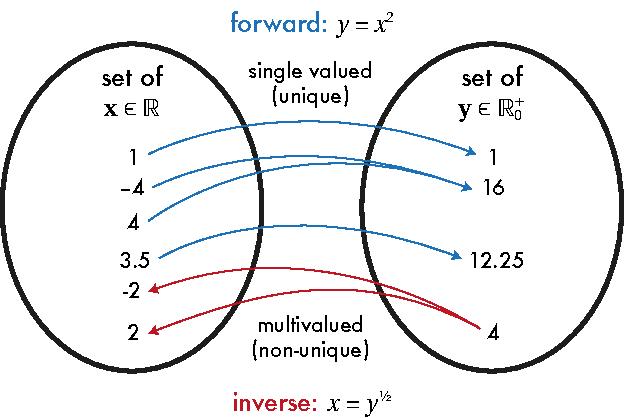
\includegraphics[]{numerical/figures/nonunique.eps}
    \caption{An example of non-uniqueness from the simple inverse of $y = x^2$.
    Solutions of $x = y^{1/2}$ are multivalued unless contrained.}
    \label{fig:nonunique}
\end{figure}

As an example of non-uniqueness, think back to our MT practical as an example where models of a conductive layer over a resistive layer shows no change in misfit (lack of sensitivity) over an extremely large range of resistivities, making them all equally likely.  In this case, the cause of non-uniqueness is a lack of sensitivity to certain model parameters due to the physics of the problem.  We can't change physics, so how can we address the ambiguity?

The shape of a misfit functional is generally smooth, but can have complexities as the model parameters change resulting in surfaces or curves that have multiple local minima (Figure~\ref{fig:misfit}).  Inversions which are iterative can get ``stuck'' within a local minima, unable to access regions with lower misfit.  Using multiple initial conditions for an inversion can occasionally help move the solution from one minima to another, but how do we tell which one is correct, certainly both cannot?  Simply choosing the lowest misfit may not be appropriate as we may be constrained by data uncertainties or the global minima may result in ``over-fitting'' the observed data.
\begin{figure}[bth]
    \centering
    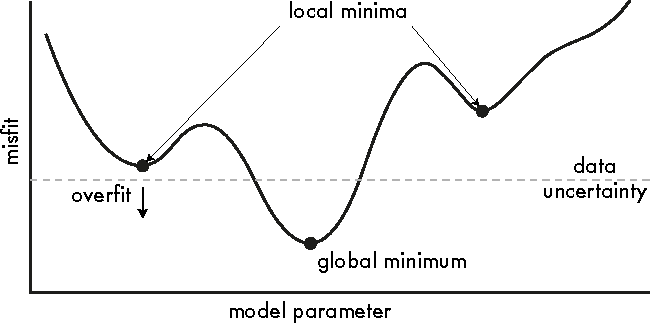
\includegraphics[]{numerical/figures/misfit_functional.pdf}
    \caption{Hypothetical misfit function.  Each point on the misfit curve
    represents a unique set of model parameters.  A misfit function may have
    multiple local minima in addition to a global minimum.  Models which sit
    below the data uncertainty overfit the data.}
    \label{fig:misfit}
\end{figure}

In some cases, it may be possible to improve sensitivity by adding data at the correct sites.  Adding additional constraints can reduce non-uniqueness, either adding another type of data with different sensitivities or geological constraints.

\subsection{Stability}
Inversion problems are notoriously unstable.  Given the wrong initial condition ``far'' from a solution may result in each successive iterative step moving increasingly further from a viable solution.  Basically the model spins out of control and the inversion will not converge.  Hence, the initial condition can affect not only the solution, but also the stability.  Another problem that can arise are models in which the values of adjacent cells increasing grow in opposite directions such that their average response at the surface may be approximately the same but the two values are increasingly divergent.  For example, imagine a resistivity cross-section that looks more like a checkerboard pattern of conductive and resistive squares rather than a geologically plausible image.  I've classified this problem as a stability issue, but it could as easily be classified as non-uniqueness as the misfit may reduce as this occurs suggesting the model fits the data but is clearly geologically implausible.

We can attempt to stabilize these problems by penalizing the misfit functional in various ways.  That is, the misfit will grow if the model strays too far from our imposed constraint in an attempt to force the inversion to take steps towards a reasonable solution rather than running away.  An analogy that sort of works is to imagine a goat tethered to a tree.
\footnote{This analogy comes from a very Russian professor, Mikhail Zhdanov, I had as a graduate student at the University of Utah.  Most of us would probably think of a tethered dog, but a goat somehow makes it so much more memorable.}
The goat can wander (misfit) anywhere between the tree and the maximum length of the rope (penalty); assuming of course that the goat doesn't eat the rope or the tree (we can only take analogies so far).  Adding these penalties doesn't always work, but it does tend to significantly improve the stability.

There are a number of misfit penalties that we can apply and we will discuss a few in greater detail in Section~\ref{sec:misfit}.  A penalty for straying too far from a prescribed model is perhaps the most closely aligned with our goat on a rope analogy.  This type of penalty best prevents the instabilities that allow models which cause misfit to grow uncontrollably.  To limit the ``checkerboard'' problem above, we can penalize the model roughness, forcing models to be smoothly varying.  The price we pay for smoothing is a difficulty in resolving boundaries that represent a step change in a model property (e.g., seismic velocity contrast between two layers).  However, there are additional method to still allow for discontinuities under certain conditions.

In addition to the stability concerns addressed above, inversions can be made unstable by the presence of a data outlier or even perhaps the smaller noisy variations in the data resulting from measurement uncertainties.  This effect can be mitigated by weighting the data by its certainty (inverse of the uncertainty) as we estimate the misfit.


\section{Misfit Functionals} \label{sec:misfit}

When developing a physical model, we require a way to quantify how well it reproduces the observed data relative to alternative models. In general, we seek a single scalar value that characterizes the mismatch between the data and a model. The mathematical expression of this mismatch is called the \emph{misfit}, a broad term for any metric used to discriminate between the performance of competing models. The choice of this metric can have a significant influence on the inversion results. A good inversion does not minimize misfit arbitrarily, but instead seeks a balance between fitting the data and producing a physically meaningful model. In selecting a metric, we implicitly introduce assumptions about noise, uncertainty, and the relative importance of different parts of the data.

To quantify misfit, we require a way to measure the size of differences between observed and predicted data. This quantification is typically accomplished using norms, which provide a measure of vector magnitude and, by extension, distance.

\ntextbox{Norms and Metrics in Inversion Theory}{
    To compare models and data, we need a way to measure how different two vectors are, such as the observed data and the predicted data. This idea is formalized using the concepts of distance, metrics, and norms, which are used to compute the misfit.

    \medskip
    \noindent\textbf{Metric (distance)} \\
    A metric is simply a measure of distance between two points or vectors. A valid distance function $d(\vb{x_1}, \vb{x_2})$ must satisfy four conditions:
    \begin{description}
        \item [Non-negativity:] distance must always be positive or zero, $d(\vb{x_1}, \vb{x_2}) \geq 0$
        \item [Identity:] the distance is zero only if the two points are identical, $d(\vb{x_1}, \vb{x_2}) = 0 \iff \vb{x_1} = \vb{x_2}$
        \item [Symmetry:] distance does not depend on order, $d(\vb{x_1}, \vb{x_2}) = d(\vb{x_2}, \vb{x_1})$
        \item [Triangle inequality:] the distance between two points is always shorter than or equal to going through a third point, $d(\vb{x_1}, \vb{x_3}) \leq d(\vb{x_1}, \vb{x_2}) + d(\vb{x_2}, \vb{x_3})$
    \end{description}

    \medskip
    \noindent\textbf{Norm (magnitude)} \\
    A norm measures the size or length of a vector, $\norm{\vb{x}} \geq 0$. Norms define a metric through
    \[
        d(\vb{x}, \vb{y}) = \norm{\vb{x} - \vb{y}},
    \]
    so that measuring misfit is equivalent to measuring distance between observed and predicted data.  For an expression to be a norm, it must satisfy properties analogous to those of a metric, including positivity, the triangle inequality, and an additional scaling property called homogeneity (defined previously in Section~\ref{sec:linearity}).

    \medskip
    \noindent\textbf{Common norms in inversion} \\
    Two norms are commonly used in inversion problems:
    \begin{description}
        \item [$L^2$-norm,] is simply the Euclidean distance, which you may remember as the Pythagorean distance for a 2-dimensional space,
        \[
            \norm{\vb{x}}_2 = \left( \sum_{i=1}^N x_i^2 \right)^{1/2}
            = (\vb{x}\T \vb{x})^{1/2}
        \]
        Note the subscript denotes the order of the norm.  This norm is the familiar straight-line distance and emphasizes larger differences more strongly. The $L^2$ norm is closely related to the arithmetic mean through the root-mean-square (RMS) value. This quantity is susceptible to outliers.

        \item [$L^1$-norm,] is the absolute distance
        \[
            \norm{\vb{x}}_1 = \sum_{i=1}^N \abs{x_i}
        \]
        This norm measures total deviation and is less sensitive to large outliers. It is closely related to the median in that minimizing an $L^1$ misfit yields a robust estimate of central tendency.
    \end{description}

    \medskip
    \noindent\textbf{Connection to inversion} \\
    In inverse problems, the misfit is simply the distance between observed and predicted data. 
    
    Because the $L^1$-norm penalizes deviations linearly, it is less sensitive to large outliers than the $L^2$-norm, which penalizes deviations quadratically. This property makes the $L^1$-norm useful when the data may contain outliers or non-Gaussian noise.
    
    Different choices of norm correspond to different ways of measuring the distance between the observed data $\vb{d}$ and the predicted data $\tilde{\vb{d}}$, and hence different definitions of what it means for a model to ``fit'' the data.
}{mathtool}\label{box:norm}

\subsection{Basic Misfit Functionals}

A common misfit functional\footnote{A functional is a function that takes a vector as an argument and returns a scalar value.}
based on the $L^2$-norm is the root-mean-square (RMS) misfit,
\begin{equation}
    \coreeq
    \phi_2 = \left( \frac{1}{N_d} 
        \sum_{i=1}^{N_d} (d_i - \tilde{d}_i)^2 \right)^{1/2},
    \label{eq:rms2}
\end{equation}
where $N_d$ is the number of data points. The RMS misfit represents the average magnitude of the residuals and corresponds to the root-mean-square value of the differences between observed and predicted data. The units of RMS are the same as the units of $\vb{d}$.

While the summation form makes the contribution of each data point explicit, it is often more convenient to express the misfit in vector form. Defining the \emph{residual} vector,
\begin{equation}
    \coreeq
    \vb{r} = \vb{d} - \tilde{\vb{d}},
\end{equation}
the $L^2$ misfit can be written as
\[
    \workeq
    \phi_2 = N_d^{-1/2} \left( \vb{r}\T \vb{r} \right)^{1/2}.
\]
or simply,
\[
    \phi_2 = N_d^{-1/2} \norm{\vb{r}}_2 .
\]

An $L^1$-norm misfit is given by
\begin{equation}
    \workeq
    \phi_1 = \frac{1}{N_d} \sum_{i=1}^{N_d} \abs{d_i - \tilde{d}_i}.
    \label{eq:rms1}
\end{equation}

The $L^1$ misfit is less influenced by large residuals and is therefore commonly used in problems such as earthquake location, where robustness to outliers is important. Note that this misfit corresponds to the mean absolute deviation, not the median.

\subsection{Weighted and Normalized Misfit}

The basic misfit functionals do not account for uncertainty in the data. In practice, it is often desirable to weight the contributions of individual data points according to their uncertainties. Data with low uncertainty are given greater influence, while noisier data contribute less.

A weighted $L^2$ misfit can be written as
\begin{equation}
    \coreeq
    \phi_2 = \left( \frac{1}{N_d} 
        \sum_{i=1}^{N_d} \frac{(d_i - \tilde{d}_i)^2}{\sigma_i^2} \right)^{1/2},
\end{equation}
where $\sigma_i$ represents the standard deviation (uncertainty) of the $i$th datum.  This expression shows explicitly that each data point is weighted according to its uncertainty, with more precise measurements contributing more strongly to the misfit. In this sense, the misfit reflects both data fit and confidence in each measurement. The weighted RMS is unitless since the elements of $\vb{d}$ are normalized by their uncertainty that has the same units.

In vector form, the weighted misfit can be written as
\begin{equation}
    \workeq
    \phi_2 = N_d^{-1/2} \norm{\vb{W}_d \vb{r}}_2 ,
\end{equation}
where $\vb{W}_d$ is a diagonal weighting matrix with elements $w_{d,ii} = 1/\sigma_i$.

\subsection{$\chi^2$ Misfit}

A commonly used related measure is the chi-squared ($\chi^2$) misfit,
\begin{equation}
    \workeq
    \chi^2 = \norm{\vb{W}_d \vb{r}}_2^2
\end{equation}
Unlike the RMS misfit, the $\chi^2$ misfit is not normalized by the number of data and therefore provides an absolute measure of misfit relative to the assumed uncertainties.

Normalizing by the number of degrees of freedom yields the reduced chi-squared,
\begin{equation}
    \chi^2_\nu = {N_{d-m}}^{-1} \norm{\vb{W}_d \vb{r}}_2^2
\end{equation}
where $N_{d-m}$ is the number of degrees of freedom (number of data minus the number of model parameters, $N_d - N_m$).

In an ideal case, we expect $\chi^2_\nu \approx 1$. Values significantly less than 1 may indicate overfitting relative to the assumed uncertainties, while values greater than 1 suggest the model does not adequately explain the data within the expected noise level.  In this sense, the chi-squared misfit provides a useful criterion for assessing whether a model fits the data at an appropriate level, rather than simply minimizing the misfit.

It is important to note that not all changes to the misfit definition affect the inversion result. The weighted RMS, $\chi^2$, and reduced $\chi^2$ misfits are related by constant scaling factors and therefore yield the same model when minimized. These forms differ only in how the misfit is normalized and interpreted.

In contrast, changing from an unweighted to a weighted misfit alters the relative importance of individual data points and generally leads to a different inversion result. More broadly, different choices of norm (e.g., $L^1$ versus $L^2$) and regularization (as we'll soon see) can lead to fundamentally different models. Only changes that alter the relative weighting of residuals will change the location of the minimum; changes in overall scaling will not.

The misfit functions introduced above provide a quantitative measure of how well a model explains the observed data. In practice, inversion methods seek to minimize this misfit by adjusting the model parameters. For linear inverse problems, this leads naturally to least-squares formulations, which will be developed in the next section. However, minimizing misfit alone is generally insufficient to define a unique or stable solution. Additional constraints on the model are typically required, and these will be introduced later.


\section{Least-Squares Inversions}

\subsection{Linear Linear Least Squares (LLSQ)}\label{sec:llsq}

Fitting lines and polynomials to data is one of the most common practices for interpreting data in many fields of science.  Most of you may be familiar with the functions that are used within a spreadsheet or other program, but may not know what it is doing behind the scenes.  Fitting a line to data is an inverse problem where we use data $y$, collected at discrete values of $x$ to determine the unknown fitting paramters, slope and $y$-intercept.

Imagine we have collected number of data (N points in all) at known locations, $x = x_1,x_2,\ldots,x_N$, resulting in observations with values, $y = y_1,y_2,\ldots,y_N$.  Assuming the data appear sufficiently linear we wish to fit a single line to all the data.  We will need to determine a slope, $m_1$, and intercept, $m_0$, which are our model, i.e., $y = m_0 + m_1 x$.  Simply fitting the data by eye is not appropriate, as it does not provide a reliable way to determine the best-fitting model or quantify uncertainty in the parameters.

We could try a range of slopes and intercepts and pick the pairs systematically or randomly and determine the one which provides the minimum misfit to the data.  Testing sets of parameters in this way is called a grid search and is essentially repeated application of the forward problem.  A grid search can be useful for mapping out the misfit surface and illustrating the sensitivities to different model parameters.  However, a grid search can be very time consuming.  As the number of of parameters grows, a grid search quickly becomes intractable.  Instead, we would rather have a way to identify the best possible model in one step.  Rather than exploring the parameter space exhaustively, we seek a method that directly identifies the model that minimizes the misfit.

One approach is to directly compute the model parameters that minimize the misfit.  The method below is called the linear least squares (LLSQ) because it minimizes the misfit of the squared difference between the data and predicted data.  Suppose we collect observations at known locations $x = x_1,x_2,\ldots,x_N$.  We choose a slope, $m_1$, and intercept, $m_0$, which yield the modeled data, $\tilde{y_i}$,
\begin{align*}
    \tilde{y}_1 &= m_0 + m_1 x_1 \\
    \tilde{y}_2 &= m_0 + m_1 x_2 \\
    \vdots \\      
    \tilde{y}_N &= m_0 + m_1 x_N ,
\end{align*}
which we can generalize as $\tilde{y}_i = m_0 + m_1 x_i$, where $x_i$ and $\tilde{y}$ are the location and estimate of the $i$-th data point.  The squared misfit of the $i$-th data point is given by,
\begin{equation*}
    r_i = y_i - \tilde{y}_i .
\end{equation*}
This individual misfit can be positive or negative indicating whether the model point is below or above the measured point.  However, we care about the total misfit (unsigned distance) from each point which is given by
\begin{equation*}
    \phi^2 = \sum_{i=1}^N r_i^2 .
\end{equation*}
Note this is an $L^2$-norm.

The minimum misfit for the $i$-th data point is a model that passes through the point $(x_i, y_i)$; though the best-fitting model for all of the data may not have a zero misfit at any given observation.  Therefore, we need to identify the set of model parameters ($m_0$ and $m_1$ in this case) which collectively provides the minimum misfit to the observations.

\ntextbox{Minimizing misfit for a line}{
    Starting from the misfit for a line, writing the model prediction as
    $\tilde{y}_i = m_0 + m_1 x_i$,
    \[
        \phi^2 = \sum_{i=1}^N (y_i - \tilde{y}_i)^2 .
    \]
    A minimum requires $\phi^2$ to be stationary with respect to \emph{each}
    parameter, so both partial derivatives vanish. Differentiating once, generically,
    with the chain rule,
    \[
        \pdv{\phi^2}{m_j} = -2 \sum_{i=1}^N (y_i - \tilde{y}_i)\,\pdv{\tilde{y}_i}{m_j}
        = 0 ,
    \]
    and for a line the basis-function derivatives are just
    $\pdv{\tilde{y}_i}{m_0} = 1$ and $\pdv{\tilde{y}_i}{m_1} = x_i$.
    The two conditions therefore say the residuals are orthogonal to each basis
    function:
    \[
        \sum (y_i - \tilde{y}_i) = 0 , \qquad
        \sum (y_i - \tilde{y}_i)\, x_i = 0 .
    \]
    Expanding $\tilde{y}_i$ gives the two \emph{normal equations} (sum limits
    $1\ldots N$ dropped on intermediate steps to reduce clutter):
    \begin{equation}
        0 = \sum_{i=1}^N y_i - m_0 N - m_1 \sum_{i=1}^N x_i ,
        \label{eq:llsq-intercept}
    \end{equation}
    \begin{equation}
        0 = \sum_{i=1}^N y_i x_i - m_0 \sum_{i=1}^N x_i - m_1 \sum_{i=1}^N x_i^2 .
        \label{eq:llsq-slope}
    \end{equation}
    To determine the optimal choices of $m_0$ and $m_1$, rearrange Equation~\ref{eq:llsq-intercept} to isolate $m_0$,
    \begin{equation}
        m_0 = \frac{1}{N} \left(\sum_{i = 1}^N y_i - m_1 \sum_{i = 1}^N x_i \right) ,
        \label{eq:llsq-b2}
    \end{equation}
    and substituting into Equation~\ref{eq:llsq-slope} and we find the optimal slope, $m$,
    \begin{align*}
        0 &= \sum y_i x_i - m \sum x_i^2 
        - \frac{1}{N} \left(\sum y_i - m_1 \sum x_i \right) \sum x_i \\
        0 &= N \sum y_i x_i - m_1 N \sum x_i^2 
        - \sum y_i \sum x_i + m_1 \left(\sum x_i \right)^2 \\
        m_1 N \sum x_i^2 - m_1 \left(\sum x_i \right)^2 &=
        N \sum y_i x_i - \sum y_i \sum x_i  ,
    \end{align*}
    and finally,
    \[
        m_1 = \frac{\displaystyle N \sum_{i = 1}^N y_i x_i - \sum_{i = 1}^N y_i \sum_{i = 1}^N x_i}
        {\displaystyle N \sum_{i = 1}^N x_i^2 - \left(\sum_{i = 1}^N x_i \right)^2} . \\
    \]
    Now that we have the optimal slope, we can input the result into Equation~\ref{eq:llsq-b2},
    \begin{align*}
        m_0 &= \frac{1}{N} \left(\sum_{i=1}^N y_i - 
        \frac{\displaystyle N \sum y_i x_i 
        - \sum y_i \sum x_i}
        {\displaystyle N \sum x_i^2 - \left(\sum x_i \right)^2}
        \sum x_i \right) \\
        m_0 &= \frac{1}{N} 
        \frac{\displaystyle N \sum y_i \sum x_i^2 
        - \sum y_i \left(\sum x_i \right)^2 
        - N \sum y_i x_i \sum x_i
        + \sum y_i \left(\sum x_i\right)^2}
        {\displaystyle N \sum x_i^2 - \left(\sum x_i \right)^2} ,
    \end{align*}
    and finally,
    \[
        m_0 = \frac{\displaystyle \sum_{i=1}^N y_i \sum_{i=1}^N x_i^2 
        - \sum_{i=1}^N y_i x_i \sum_{i=1}^N x_i}
        {\displaystyle N \sum_{i=1}^N x_i^2 - \left(\sum_{i=1}^N x_i \right)^2} .
    \]
    The variance for each model parameters is estimated by
    \begin{align*}
        \sigma_{m_0}^2 &= \frac{\displaystyle \sum_{i=1}^N x_i^2 \sum_{i=1}^N \phi_i^2}
        {\displaystyle (N - 2) 
        \left[ N \sum_{i=1}^N x_i^2 - \left(\sum_{i=1}^N x_i \right)^2 \right]} , \\
        \sigma_{m_1}^2 &= \frac{\displaystyle N \sum_{i=1}^N \phi_i^2}
        {\displaystyle (N - 2) 
        \left[ N \sum_{i=1}^N x_i^2 - \left(\sum_{i=1}^N x_i \right)^2 \right]} ,
    \end{align*}

    These equations show that the optimal parameters are determined by enforcing that the residuals are uncorrelated with the model basis functions.
}{aside}\label{box:llsq}

The minimization method in Box~\ref{box:llsq} is tedious. Additionally, it is a bit difficult, though possible, to extend to polynomials as well as lines. However, all the sums and terms make it fairly cluttered.  While this scalar derivation is instructive, it quickly becomes cumbersome for more complex models. A more compact and general formulation can be obtained using linear algebra.  Consider the equations of a line now written in matrix form,
\[
    \underbrace{
        \begin{bmatrix}
            1 & x_1 \\
            1 & x_2 \\
            \vdots & \vdots \\
            1 & x_N
        \end{bmatrix}
    }_{\vb{A}}
    \underbrace{
        \begin{bmatrix}
            m_0 \\
            m_1 \\
        \end{bmatrix}
    }_{\vb{m}} =
    \underbrace{
        \begin{bmatrix}
            y_1 \\
            y_2 \\
            \vdots \\
            y_N
        \end{bmatrix}
    }_{\vb{d}} ,
\]
which we can write as simply
\[
    \vb{A} \vb{m} = \vb{d} .
\]
Solving $\vb{A}\vb{m} = \vb{d}$ directly would require inverting $\vb{A}$, i.e., $\vb{A}^{-1}$. But computing the inverse of $\vb{A}$ directly is generally not possible because $\vb{A}$ is not square. Instead, we seek a generalized inverse that provides the best-fitting solution. This generalization requires approximating the inverse of $\vb{A}$,
\[
    \vb{m} = \vb{A}^+ \vb{d} ,
\]
where $\vb{A}^+$ is the pseudo-inverse.  The end result will be the same
solution for LLSQ as above, but in matrix form.  By multiplying
both sides by the transpose of $\vb{A}$,
\[
    \vb{A}\T \vb{A} \vb{m} = \vb{A}\T \vb{d},
\]
we create a square matrix, $\vb{A}\T \vb{A}$. Assuming this matrix is nonsingular, it can be inverted, resulting in the LLSq solution
\begin{equation}
    \coreeq
    \vb{m} = (\vb{A}\T \vb{A})^{-1} \vb{A}\T \vb{d} .
    \label{eq:llsq_solution}
\end{equation}
Hence, the pseudo-inverse, $\vb{A}^+$, given by
\begin{equation}
    \coreeq
    \vb{A}^+ = (\vb{A}\T \vb{A})^{-1} \vb{A}\T ,
    \label{eq:llsq_pseudoinverse}
\end{equation}
performs the inverse that we otherwise would have done if possible.  This matrix solution is the LLSQ inversion and, as I'm sure you will agree, more compact than the purely algebraic form.

Once we have $\vb{m}$, we can then compute the pseudodata,
\[
    \vb{A} \vb{m} = \tilde{\vb{d}},
\]
and the misfit from the residuals ($\vb{r} = \vb{d} - \tilde{\vb{d}}$),
\[
    \phi = \norm{\vb{r}} .
\]

Equation~\ref{eq:llsq_solution} provides a solution, not necessarily the unique or most appropriate solution.  Different definitions of misfit and additional constraints can lead to alternative solutions that may be more meaningful or physically realistic.  For instance, the solution above does not take into account uncertainties in the data and all data are given equal weight.  It is rarely the case with real data that our uncertainties and errors are all the same.  Therefore, we need a way to incorporate these uncertainties by giving greater weight to the more certain data and less weight to the more uncertain data.

\subsection{Weighted Linear Least Squares (WLLSQ)}

In the previous section, we assumed that all data were equally reliable. In practice, measurements often have different levels of uncertainty, which must be accounted for in the inversion.

To weight the data based on their uncertainty, we redefine our misfit to include estimates of the data uncertainties,
\begin{equation}
    \phi = \norm{\vb{W}_d \vb{r}} ,
\end{equation}
where $\vb{W}_d$ with diagonals defined by $1/\sigma_i$.  To incorporate these uncertainties into the matrix formulation, we scale both sides of the forward equation, i.e.,
\begin{equation}
    \vb{W_d} \vb{A} \vb{m} = \vb{W_d} \vb{d} ,
\end{equation}
where $\vb{W_d}$ is the weighting matrix, defined by
\begin{equation}
    \vb{W_d} =
    \begin{bmatrix}
        \sigma_1^{-1} & 0 & 0 & \dots & 0 \\
        0 & \sigma_2^{-1} & 0 & \dots & 0 \\
        0 & 0 & \sigma_3^{-1} & \dots & 0 \\
        \vdots & & & \ddots & \vdots \\
        0 & 0 & 0 & \dots & \sigma_N^{-1} \\
    \end{bmatrix} .
\end{equation}
The weighting matrix is diagonal---zero everywhere except the diagonal elements---so each data point is scaled independently according to its uncertainty.  Following a similar procedure now as we did before we can show that the solution to the weighted LLSQ problem is given by
\begin{equation}
    \vb{m} = (\vb{A}\T \vb{W_d}^2 \vb{A})^{-1} \vb{A}\T \vb{W_d}^2 \vb{d} .
\end{equation}

Alternatively, if we redefine the operator matrix and data vector as
\[
    \vb{A}_w = \vb{W}_d \vb{A}, \quad \vb{d}_w = \vb{W}_d \vb{d} ,
\]
we can write the WLLSQ solution as
\[
    \vb{m} = (\vb{A}_w\T \vb{A}_w)^{-1} \vb{A}_w\T \vb{d}_w .
\]
We have implicitly rewritten the weighted misfit in terms of a scaled residual $\vb{W}_d \vb{r}$. In this formulation, the weighting can be interpreted as rescaling the data so that all measurements have comparable uncertainty, allowing the least-squares problem to retain the same algebraic form as the unweighted case (Equation~\ref{eq:llsq_solution}).

This formulation is both mathematically compact and computationally efficient. Since many modern programming languages support linear algebra operations directly (e.g., MATLAB, Python, Julia), implementing inversion methods in this form is straightforward.

\subsubsection{Model Parameter Uncertainty}

The weighted formulation allows us to estimate uncertainty in the model parameters. The covariance matrix of the model is given by
\begin{equation}
    \vb{C}_m = (\vb{A}\T \vb{W_d}^2 \vb{A})^{-1},
\end{equation}
which describes how uncertainties in the data propagate into uncertainties in the model.

The diagonal elements of $\vb{C}_m$ represent the variances of the individual model parameters,
\[
    \sigma_{m_i}^2 = (\vb{C}_m)_{ii},
\]
while the off-diagonal elements describe correlations between model parameters.  This expression generalizes the scalar uncertainty formulas derived in the previous section and provides a more complete description of model uncertainty when data have varying levels of reliability.

Once the model covariance matrix is determined, we can estimate uncertainty in each model parameter. The vector of model variances can be written compactly as
\[
    \vb{\sigma}_m^2 = \diag (\vb{C}_m),
\]
with standard deviations given by
\[
    \vb{\sigma}_m = \sqrt{\diag(\vb{C}_m)},
\]
where the square root is taken element-wise.

Assuming the parameter estimates are approximately normally distributed, a 95\% confidence interval for the $i$th model parameter can be written as
\[
    \vb{m} \pm 1.96\,\bm{\sigma}_m.
\]
This expression is interpreted component-wise, so that the confidence interval is applied independently to each model parameter.  More generally, for finite data sets, the confidence interval can be expressed using the Student's $t$-distribution,
\[
    \vb{m} \pm t_{\alpha/2,\nu} \,\bm{\sigma}_m,
\]
where $\nu = N_d - N_m$ is the number of degrees of freedom. For large $\nu$, $t_{\alpha/2,\nu} \approx 1.96$, and the normal approximation is appropriate.

These confidence intervals provide a quantitative measure of how uncertainty in the data propagates into uncertainty in the estimated model parameters.  It is important to note that these uncertainties depend on the assumed data uncertainties and the model parameterization.

It is worth noting that these expressions also reduce naturally to the unweighted case. If all data are assumed to have equal uncertainty, the weighting matrix $\vb{W}_d$ becomes the identity matrix, and the weighted formulation simplifies to the standard linear least squares result. In this case, the model covariance reduces to $\vb{C}_m = \sigma^2 (\vb{A}\T \vb{A})^{-1}$, consistent with the expressions derived previously.

\section{Constrained Inversions}

\subsection{Motivation and Types of Constraints}
Inverse models do not always return geologically realistic solutions. These unrealistic models can arise for several reasons: the mathematics may admit solutions that are not physically meaningful, the problem may be poorly determined, or the data may be contaminated by noise.  A classic example is the $\text{D}^{+}$ magnetotelluric model, which produces layers of infinite resistivity separated by infinitesimally thin layers with finite conductance. While these models satisfy the governing equations, they are not physically plausible given the properties of geologic materials.

To obtain more geologically realistic results, we must restrict the set of allowable models. Regularization provides a framework for imposing such constraints on the inversion.  Regularization modifies the inverse problem by adding a penalty term that discourages undesirable model characteristics. In practice, this means prioritizing certain features in the model, such as smoothness, small amplitude, or structural simplicity. These constraints are introduced by modifying the misfit functional to penalize specific behaviors.  The table below lists a few of the ways such constraints are added.
\begin{table}
    \centering
    \caption{Methods for adding constraints to inversions.}
    \label{tab:regularization}
    \begin{tabularx}{\textwidth}{@{}lcXX@{}}
        \toprule
        \textbf{Constraint} &
        \textbf{Functional}, $\phi_m$ &
        \textbf{Effect} &
        \textbf{Typical use} \\
        \midrule
        damping (Tikhonov) &
        $\norm{\vb{m}}^2$ &
        small amplitude, minimum-energy models &
        stabilizes ill-conditioned problems, suppresses unrealistically large values \\

        smoothing &
        $\norm{\vb{L}\vb{m}}^2$ &
        smooth structure, spatial continuity, suppresses oscillations &
        suppresses noise amplification and promotes geologically continuous structure \\

        Occam &
        Section~\ref{sec:occam} &
        simplest (smoothest) model consistent with the data &
        minimizes unnecessary structure and avoids overfitting \\

        total variation &
        $\norm{\grad{\vb{m}}}_1$ &
        blocky structure, sharp boundaries, piecewise-constant models &
        imaging, fault recognition, sharp geologic boundaries \\

        focusing &
        $\norm{\vb{m}}_1$ &
        prioritizes zero values (sparsity), compact anomalies &
        localized targets, compact sources, parsimonious models \\

        minimum structure &
        $\sum_i \frac{m_i^2}{m_i^2 + \epsilon^2}$ &
        discrete bodies, sharp anomalies &
        ore deposits, potential fields, localized conductivity or density anomalies \\

        bounded &
        $m_{\min} \le m \le m_{\max}$ &
        constrained inversion within allowable ranges &
        positive- or negative-only values, physical property ranges, monotonicity, thermodynamic constraints \\

        coupled &
        $\grad{\vb{m}_1} \times \grad{\vb{m}_2} \approx 0$ &
        structurally similar coupled models &
        structurally correlated models, petrophysical covariance, joint inversion \\

        temporal &
        $\norm{\vb{m}_t - \vb{m}_{t-1}}^2$ &
        temporal smoothing, stable evolution &
        suppresses unrealistic temporal variability in time-lapse inversions \\
        \bottomrule
    \end{tabularx}
\end{table}

For a weighted least-squares problem, the data misfit can be written as
\[
    \phi_d(\vb{m}) = \norm{\vb{W}_d (\vb{d} - \vb{A}\vb{m})}_2^2.
\]

Previously we have focused on the misfit provided by the data $\phi_d$.  Regularization introduces an additional penalty term, $\phi_m$, leading to an objective function of the form
\begin{equation}
    \coreeq
    \Phi(\vb{m}) = \phi_d(\vb{m}) + \lambda \phi_m(\vb{m}) , 
\end{equation}
where $\lambda$ is the regularization hyperparameterthat controls the trade-off between fitting the data and satisfying the model constraints. The choice of $\phi_m$ depends on the desired characteristics of the model.


\subsection{Damping (Tikhonov regularization)}

Least-squares solutions, even when weighted by data uncertainty, do not always produce geologically reasonable models. In particular, poorly constrained parameters may take on unrealistically large values while still fitting the data adequately. Damping provides a simple and effective way to stabilize the inversion by penalizing the overall magnitude of the model parameters.

In its simplest form, damping (also known as zero-order Tikhonov regularization) penalizes deviations of the model from zero,
\[
    \phi_m(\vb{m}) = \norm{\vb{m}}_2^2.
\]
This favors minimum-energy solutions and suppresses large-amplitude features that are not required by the data.

More generally, it is often preferable to damp the model relative to an \textit{a priori}\footnote{The Latin \textit{a priori} means ``from what is earlier'' and is frequently used in statistics and sciences to mean prior knowledge.  In this case the \textit{a priori} model may be based on prior assumptions or genuine knowledge about a system (reference model), or it could simply be a simple model like a uniform half-space.}
or reference model, $\vb{m}_\text{ref}$, rather than zero. In this case, the model penalty is written as
\[
    \phi_m(\vb{m}) = \norm{\vb{m} - \vb{m}_\text{ref}}_2^2,
\]
which encourages solutions that remain close to the reference model unless the data demand otherwise. The Russian professor who taught me inverse theory used the analogy of a goat tethered to a stake to describe this form of regularization. The goat may wander freely, but the farther it moves from the stake, the stronger the restoring force becomes. In this sense, damping penalizes deviation from the reference model rather than imposing a hard constraint.

Using the weighted least-squares formulation introduced earlier, the regularized objective function becomes
\begin{equation}
    \workeq
    \Phi(\vb{m}) = \underbrace{\norm{\vb{r}_w}_2^2}_{\phi_d} + \lambda \underbrace{\norm{\vb{m} - \vb{m}_\text{ref}}_2^2}_{\phi_m},
\end{equation}
where $\lambda$ controls the strength of the damping relative to the data misfit.

Minimizing this objective function yields the normal equations
\[
    (\vb{A}_w\T \vb{A}_w + \lambda \vb{I}) \vb{m} =
    \vb{A}_w\T \vb{d}_w + \lambda \vb{m}_\text{ref}.
\]
The additional term $\lambda \vb{I}$ stabilizes the inversion and suppresses large model amplitudes, particularly in poorly constrained problems.

Solving for the model parameters gives
\begin{equation}
    \workeq
    \vb{m} = (\vb{A}_w\T \vb{A}_w + \lambda \vb{I})^{-1}
    \left(
        \vb{A}_w\T \vb{d}_w + \lambda \vb{m}_\text{ref}
    \right).
\end{equation}

\subsection{Smoothing}

Least-squares solutions, even when stabilized by damping, can still exhibit unrealistic spatial variability. In many inverse problems, especially those involving distributed Earth properties, the data do not contain sufficient information to resolve sharp variations between neighboring model parameters. As a result, small-scale oscillations may appear in the solution that fit the data but have no geological significance.

Smoothing constraints address this problem by penalizing spatial variability in the model rather than its overall magnitude. In effect, smoothing expresses the assumption that subsurface properties vary gradually unless the data provide strong evidence otherwise. This reflects both geological expectation and the limited resolving power of most geophysical measurements.

Smoothing is introduced by defining a model penalty that measures roughness rather than amplitude. In operator form, the model penalty is written as
\[
    \phi_m(\vb{m}) = \norm{\vb{L}\vb{m}}_2^2,
\]
where $\vb{L}$ is a discrete derivative operator that measures spatial variation in the model.

Using the weighted least-squares formulation introduced earlier, the regularized objective function becomes
\begin{equation}
    \Phi(\vb{m}) = \norm{\vb{r}_w}_2^2 + \lambda \norm{\vb{L}\vb{m}}_2^2.
\end{equation}

Minimizing this objective function yields the normal equations
\[
    (\vb{A}_w\T \vb{A}_w + \lambda \vb{L}\T \vb{L}) \vb{m}
    = \vb{A}_w\T \vb{d}_w,
\]
with solution
\begin{equation}
    \vb{m} = (\vb{A}_w\T \vb{A}_w + \lambda \vb{L}\T \vb{L})^{-1}
    \vb{A}_w\T \vb{d}_w.
\end{equation}

Compared with damping, smoothing replaces the identity matrix with $\vb{L}\T\vb{L}$, so that the penalty acts on spatial derivatives of the model rather than on the model itself.

Conceptually, smoothing corresponds to penalizing derivatives of a continuous model. A first-derivative (gradient) penalty can be written as
\begin{equation}
    \phi_m(m) = \int \norm{\grad m(\vb{x})}^2 \, \dd{\vb{x}},
\end{equation}
which discourages rapid spatial changes and promotes smoothly varying structure.

A second-derivative (curvature) penalty takes the form
\begin{equation}
    \phi_m(m) = \int \norm{\laplacian m(\vb{x})}^2 \, \dd{\vb{x}},
\end{equation}
which suppresses variations in gradient and produces even smoother models.

These expressions are useful for understanding the intent of smoothing constraints, but they are not evaluated directly in numerical inversions.

In practice, the model is discretized into a finite set of parameters,
\[
    \vb{m} = \begin{bmatrix} m_1 & m_2 & \cdots & m_N \end{bmatrix}\T,
\]
and spatial derivatives are approximated using finite differences (Chapter~\ref{ch:finitediff}).

A first-derivative (gradient) operator can be written as
\begin{equation}
    \vb{L}_1 =
    \begin{bmatrix}
        -1 & 1 & 0 & \cdots & 0 \\
        0 & -1 & 1 & \cdots & 0 \\
        \vdots & & \ddots & \ddots & \vdots \\
        0 & \cdots & 0 & -1 & 1
    \end{bmatrix},
\end{equation}
with corresponding penalty
\[
    \phi_m = \norm{\vb{L}_1 \vb{m}}_2^2,
\]
which penalizes differences between adjacent model parameters and promotes piecewise smooth structure.

A second-derivative (curvature) operator can be written as
\begin{equation}
    \vb{L}_2 =
    \begin{bmatrix}
        1 & -2 & 1 & 0 & \cdots & 0 \\
        0 & 1 & -2 & 1 & \cdots & 0 \\
        \vdots & & \ddots & \ddots & \ddots & \vdots \\
        0 & \cdots & 0 & 1 & -2 & 1
    \end{bmatrix},
\end{equation}
with penalty
\[
    \phi_m = \norm{\vb{L}_2 \vb{m}}_2^2.
\]
Second-derivative smoothing suppresses curvature and typically produces smoother models than first-derivative constraints.

In higher dimensions, analogous finite-difference operators are constructed for each spatial direction, and the total smoothing constraint is formed by combining the corresponding operators.

The choice between first- and second-derivative smoothing has important consequences for the resulting model. First-derivative smoothing allows linear trends and gradual changes, whereas second-derivative smoothing strongly suppresses curvature and produces very smooth models.

In both cases, smoothing reflects the limited resolving power of geophysical data. Sharp boundaries may exist in the Earth, but the data often cannot locate them precisely. Smoothing therefore represents a statement about what the data can reliably resolve, rather than a claim about the true structure of the subsurface.

This perspective provides a natural bridge to Occam inversion, which formalizes the idea of selecting the simplest model—often the smoothest—that is consistent with the data.

\subsection{Choosing the Regularization Parameter, $\lambda$}

Regularization introduces an additional degree of freedom into the inverse problem through the parameter $\lambda$, which controls the trade-off between fitting the data and enforcing model constraints. Small values of $\lambda$ prioritize data fit and may produce rough or unstable models, while large values emphasize model smoothness at the expense of fitting the observations.

There is no single universally optimal choice of $\lambda$, but several strategies exist to guide its selection.

A common diagnostic tool is the \emph{L-curve}, which plots the model penalty $\phi_m(\vb{m})$ against the data misfit $\phi_d(\vb{m})$ for a range of $\lambda$ values. Such plots often form an L-shaped curve, reflecting a trade-off between data fit and model complexity. The corner of the L-curve corresponds to a solution that balances these competing objectives and is often taken as a reasonable choice for $\lambda$.

The L-curve does not provide an automatic solution, but it offers valuable insight into how sensitive the inversion is to the choice of regularization and clarifies the consequences of prioritizing either data fit or model simplicity.

Although L-curves are often used to visualize the trade-off between data misfit and model roughness, Occam inversion does not explicitly identify the corner of an L-curve as we'll see below.

\subsection{Bounded Constraints}

In many inverse problems, model parameters are subject to physical bounds, such as positivity or known limits,
\[
    \vb{m}_{\min} \le \vb{m} \le \vb{m}_{\max}.
\]
Incorporating these constraints ensures that inversion results remain physically meaningful.

Several approaches are commonly used to enforce bounded constraints.

1.\; One approach is to reparameterize the model so that the bounds are satisfied automatically. For example,
\[
    m = \exp(u)
\]
enforces positivity, while more general transformations can map unconstrained variables to bounded intervals. These transformations allow standard inversion methods to be applied but may introduce additional nonlinearity.

2.\; Alternatively, constraints can be enforced by projecting the model back into the feasible region after each update. Given a trial model,
\[
    \vb{m}_{\text{trial}} = \vb{m}_i + \Delta \vb{m},
\]
each parameter is adjusted to satisfy the bounds,
\[
    m_j =
    \begin{cases}
        m_{\min}, & m_j < m_{\min} \\
        m_{\max}, & m_j > m_{\max} \\
        m_j, & \text{otherwise}.
    \end{cases}
\]
This approach is simple and compatible with Gauss--Newton and Levenberg--Marquardt methods, although it may affect convergence near the boundaries.

3.\; More rigorous approaches treat the bounds as part of the optimization problem and solve
\[
    \min \Phi(\vb{m}) \quad \text{subject to constraints}.
\]
Methods such as active-set or interior-point algorithms modify the update step to ensure that constraints are satisfied throughout the inversion. With their rigor comes greater difficulty to implement.

Bounded constraints restrict the admissible model space and help prevent nonphysical solutions. They are particularly important in nonlinear inversion, where large updates may otherwise produce unrealistic parameter values. In practice, a balance is required between enforcing constraints and maintaining smooth convergence of the inversion.

\subsection{Occam Inversion}\label{sec:occam}

William of Occam was a 14th-century English philosopher best known for the principle known as Occam's razor: among competing explanations that are consistent with the observations, the simplest should be preferred.

Occam inversion, developed by \citet{Constable_etal1987}, formalizes this idea in the context of inverse problems. Rather than attempting to determine a single ``true'' model, the method seeks the simplest model—typically the smoothest—that is consistent with the observed data within an acceptable level of misfit.

In this sense, Occam inversion can be viewed as a systematic approach to selecting the regularization parameter. Instead of fixing $\lambda$ directly, the method specifies an acceptable data misfit, usually consistent with the expected noise level (e.g., $\chi_\nu^2 \approx 1$), and then identifies the smoothest model that satisfies this criterion.

Although L-curves are often used to visualize the trade-off between data misfit and model roughness, Occam inversion does not explicitly identify the geometric corner of an L-curve. Instead, the solution typically lies near the L-curve corner as a consequence of enforcing the misfit criterion, rather than as the result of a curvature optimization.

Although Occam inversion is often introduced as a constrained optimization problem,
\begin{equation}
    \min_{\vb{m}} \; \norm{\vb{L}\vb{m}}_2^2
    \quad \text{subject to} \quad
    \phi_d(\vb{m}) = \phi_d^*,
\end{equation}
it is typically implemented by solving a sequence of regularized least-squares problems with different values of the regularization parameter $\lambda$.

Specifically, for a given value of $\lambda$, the model is obtained by minimizing the penalized objective function
\begin{equation}
    \Phi(\vb{m}) =
    \norm{\vb{W}_d(\vb{d} - \vb{A}\vb{m})}_2^2
    + \lambda \norm{\vb{L}\vb{m}}_2^2,
\end{equation}
which leads to the linear system
\begin{equation}
    (\vb{A}_w\T \vb{A}_w + \lambda \vb{L}\T \vb{L}) \vb{m}
    = \vb{A}_w\T \vb{d}_w.
\end{equation}
The Occam method was originally formulated with $\phi{m}$ determined using roughness, but in theory a wide variety of formulations are possible.

The resulting model $\vb{m}(\lambda)$ has an associated data misfit $\phi_d(\vb{m}(\lambda))$ and model roughness $\phi_m(\vb{m}(\lambda))$. Occam inversion proceeds by adjusting $\lambda$ until the data misfit satisfies the target criterion
\begin{equation}
    \phi_d(\vb{m}) \approx \phi_d^*,
\end{equation}
where $\phi_d^*$ is typically chosen so that the reduced chi-squared statistic satisfies $\chi_\nu^2 \approx 1$.

From this perspective, Occam inversion can be viewed as an automated procedure for selecting $\lambda$ based on a statistically meaningful misfit criterion.

In practice, this is achieved using an iterative search over $\lambda$, for example:
\begin{enumerate}
    \item Choose an initial value of $\lambda$.
    \item Solve the regularized least-squares system for $\vb{m}(\lambda)$.
    \item Evaluate the resulting data misfit $\phi_d(\vb{m}(\lambda))$.
    \item If $\phi_d > \phi_d^*$, decrease $\lambda$; if $\phi_d < \phi_d^*$, increase $\lambda$.
    \item Repeat until the misfit criterion is satisfied within a specified tolerance.
\end{enumerate}

This procedure yields the smoothest model that fits the data to the prescribed level and avoids the ambiguity associated with selecting the corner of an L-curve explicitly. The Occam solution typically lies near the L-curve corner, but this location is a consequence of the misfit constraint rather than a geometric optimization of the curve itself.

The resulting model is not unique, but it avoids unnecessary structure and provides a stable and interpretable solution. This formulation highlights a key principle of inversion: the goal is not to determine a unique model, but to identify a class of models that balance data fit and model simplicity.

The Occam inversion method is widely used in geophysical applications, particularly in electromagnetic and seismic inversion, where smooth models often provide the most reliable representation of subsurface structure.


\section{Non-linear Inverse Problems}

A forward problem is nonlinear when it does not satisfy the conditions of linearity.   In geophysics, many inverse problems are nonlinear, not necessarily because the governing physics is complex, but because model parameters influence the observations in a nonlinear manner.   Common sources of nonlinearity include:
\begin{description}
    \item [Geometry:]
    When observations depend on the spatial location, shape, or extent of structures, such as depths to interfaces or source positions. Geometry is often the dominant source of nonlinearity in geophysical problems.

    \item [Boundary conditions:]
    When the behavior of a field depends on unknown or changing boundaries, such as topography, layer interfaces, or free surfaces.

    \item [Parameter coupling:]
    When two or more parameters influence the data in a multiplicative or otherwise inseparable way, making it impossible to isolate their individual effects directly.

    \item [Nonlinear physical laws:]
    When the governing equations themselves are nonlinear in the parameters of interest, such as velocity-dependent ray paths or temperature-dependent material properties.

    \item [Implicit parameter dependence:]
    When model parameters affect the data indirectly through intermediate quantities, such as paths, sensitivities, or state variables that themselves depend on the model.
\end{description}

Unlike linear problems, nonlinear inverse problems cannot be solved in a single step. Instead, they are addressed through iterative methods that progressively refine a model estimate.

\subsection{Linearization}

In some cases, nonlinear relationships can be transformed into linear ones.  These transforms allow us to then solve for the transformed model parameters using linear least squares and solved in a single step.  Then to find the model parameters one simply needs to perform the inverse transform.

For example, if we wish to model electrical conductivity measurements on a rock at several temperature conditions, we typically us the following non-linear equation:
\begin{equation*}
    \sigma = \sigma_0 \exp \left( -\frac{H} {kT} \right) ,
\end{equation*}
where $\sigma_0$ and $H$ are unknown model parameters, $T$ is controlled, and $\sigma$ is the data.  We can transform the non-linear equation above into a linear equation by simply taking the natural logarithm of both sides,
\begin{align*}
    \log \sigma &= \log \left[ \sigma_0\exp \left( -\frac{H} {kT} \right) \right] \\
    \underbrace{\log \sigma}_{y} &= \underbrace{\log \sigma_0}_{m_0} - \underbrace{\frac{H}{k}}_{m_2} \underbrace{T^{-1}}_{x} .
\end{align*}
By redefining one of our model parameters as above, we achieve a
linear equation that can be solved using an LLSQ approach. Note that in this example, we find that the values for $H$ and $k$ are not independent.\footnote{While $H$ and $k$ are not independent, $k$ is the Boltzmann constant so we can actually determine $H$ in this case.}

However, most nonlinear problems cannot be linearized analytically.  More generally, nonlinear forward problems are linearized locally about a reference model using a first-order Taylor expansion,
\[
    \Fop(\vb{m}) \approx \Fop(\vb{m}_i)
    + \vb{J}(\vb{m}_i)(\vb{m} - \vb{m}_i),
\]
where $\vb{J}$ is the Jacobian matrix. This linear approximation is valid only in the neighborhood of $\vb{m}_i$, motivating the use of iterative solution methods.

\subsection{Gauss--Newton Method}\label{sec:newton}

Newton's method provides a general framework for minimizing nonlinear objective functions by locally approximating them with a quadratic. The Gauss--Newton method is a practical approximation of Newton's method that avoids explicit evaluation of second derivatives while retaining much of its efficiency.

The Gauss--Newton step can be interpreted in two equivalent ways. 
In the first, the objective function is approximated locally by a quadratic and the minimum of this approximation defines the update.  In the second, the method seeks the root of the gradient, $\grad \Phi = 0$, by applying Newton--Raphson to the gradient itself. 
These two perspectives lead to identical update equations but offer different geometric interpretations (Figure~\ref{fig:gauss_newton}).

For a weighted least-squares objective function,
\[
    \Phi(\vb{m}) = \norm{\vb{W}_d (\vb{d} - \Fop(\vb{m}))}_2^2,
\]
the Gauss--Newton method proceeds by linearizing the forward problem about the current model $\vb{m}_i$.

Letting
\[
    \tilde{\vb{d}} = \Fop(\vb{m}_i), \quad
    \vb{r} = \vb{d} - \tilde{\vb{d}},
\]
and defining the Jacobian
\[
    J_{ij} = \pdv{d_i}{m_j},
\]
the forward problem can be approximated as
\[
    \vb{d} \approx \tilde{\vb{d}} + \vb{J} \, \Delta \vb{m}.
\]

Minimizing the objective with respect to $\Delta \vb{m}$ leads to the linear system
\begin{equation}
    (\vb{J}\T \vb{W}_d^2 \vb{J}) \, \Delta \vb{m}
    = \vb{J}\T \vb{W}_d^2 \vb{r}.
    \label{eq:gn_basic}
\end{equation}

The model is then updated according to
\[
    \vb{m}_{i+1} = \vb{m}_i + \Delta \vb{m}.
\]

\medskip
\noindent\textbf{Role of the Jacobian} \\

The Jacobian matrix plays a central role in nonlinear inversion. Its elements,
\[
    J_{ij} = \pdv{d_i}{m_j},
\]
measure how each datum responds to a change in each model parameter.

\begin{itemize}
    \item Each \emph{row} of $\vb{J}$ describes how a single observation depends on all model parameters.
    \item Each \emph{column} describes how a single parameter influences all data.
\end{itemize}

In this sense, the Jacobian generalizes the forward operator $\vb{A}$ from linear inversion, but is evaluated at the current model and therefore changes during the inversion.

Because $\vb{J}$ depends on $\vb{m}_i$, the Gauss--Newton method solves a sequence of linearized inverse problems, updating the sensitivities at each iteration.

\medskip
\noindent\textbf{Weighted formulation} \\

In practice, data are weighted by their uncertainties. Defining
\[
    \vb{J}_w = \vb{W}_d \vb{J}, \qquad
    \vb{r}_w = \vb{W}_d \vb{r},
\]
Equation~\ref{eq:gn_basic} becomes
\[
    (\vb{J}_w\T \vb{J}_w) \, \Delta \vb{m}
    = \vb{J}_w\T \vb{r}_w,
\]
which has the same form as the weighted least-squares solution derived earlier, but now applies to a locally linearized problem.

\medskip
\noindent\textbf{Interpretation} \\

The Gauss--Newton method can be interpreted as solving a sequence of linear least-squares problems, each constructed from a local approximation to the nonlinear forward model. When the objective function is well approximated by a quadratic near the current model, the method converges rapidly. However, when the approximation is poor, the update may overshoot or converge to an unintended minimum, motivating the use of damping, regularization, or step-size control in practice.

\ntextbox{Extended derivation of the Gauss--Newton method}{
    Newton's method approximates the objective function locally by a quadratic in model space and computes a model update that aims to reach the local minimum in a single step. This large-step behavior can be efficient when the approximation is accurate, but it can also be unstable and may cause the solution to overshoot or converge to a different minimum.  In contrast, steepest descent (Section~\ref{sec:steepest})methods use only gradient information and take smaller steps, making them more stable but often slower to converge.  The Gauss--Newton method is an approximation of Newton's method, which we'll get to towards the end of the derivation.

    \medskip
    \noindent\textbf{Newton's Method} \\
    We start by expanding the objective function, $\Phi(\vb{m} + \Delta \vb{m})$, using a Taylor series about the current model $\vb{m}$:
    \[
        \Phi(\vb{m}+\Delta \vb{m}) =
        \Phi(\vb{m})
        + \pdv{\Phi}{\vb{m}}\T \Delta\vb{m}
        + \frac{1}{2} \Delta\vb{m}\T \pdv[2]{\Phi}{\vb{m}} \Delta\vb{m}
        + \varepsilon.
    \]

    Here, the first derivative corresponds to the gradient of the objective function,
    \[
        \pdv{\Phi}{\vb{m}} = \grad_{\vb{m}} \Phi(\vb{m}) =
        \begin{bmatrix}
            \pdv{\Phi}{m_1} \\
            \vdots \\
            \pdv{\Phi}{m_M}
        \end{bmatrix} .
    \]
    where $\grad_{\vb{m}}$ denotes the gradient with respect to the model parameters.  For the remaining derivation, we'll revert to $\grad$ as it is standard notation.  The second derivative defines the Hessian matrix,
    \[
        \pdv[2]{\Phi}{\vb{m}} = \vb{H} =
        \begin{bmatrix}
            \pdv{\Phi}{m_1}{m_1} & \cdots & \pdv{\Phi}{m_1}{m_M} \\
            \vdots & \ddots & \vdots \\
            \pdv{\Phi}{m_M}{m_1} & \cdots & \pdv{\Phi}{m_M}{m_M}
        \end{bmatrix}.
    \]

    Neglecting higher-order terms, the Taylor expansion becomes
    \[
        \Phi(\vb{m} + \Delta\vb{m})
        \approx
        \Phi(\vb{m})
        + \grad\Phi\T \Delta\vb{m}
        + \frac{1}{2} \Delta\vb{m}\T \vb{H} \Delta\vb{m}.
    \]

    Newton's method chooses $\Delta\vb{m}$ to minimize this quadratic approximation. Taking the derivative with respect to $\Delta\vb{m}$ gives
    \[
        \grad \Phi + \vb{H} \Delta\vb{m} = 0,
    \]
    so that
    \[
        \Delta\vb{m} = - \vb{H}^{-1} \grad \Phi.
    \]
    The update is therefore
    \begin{equation}
        \vb{m}_{i+1} = \vb{m}_i + \Delta\vb{m}
        = \vb{m}_i - \vb{H}^{-1} \grad \Phi.
        \label{eq:newton_update}
    \end{equation}

    \medskip
    \noindent\textbf{Gradient and Hessian for least-squares objectives} \\
    Let the objective function be
    \[
        \Phi(\vb{m}) = \norm{\vb{r}}_2^2 = \vb{r}\T \vb{r},
    \]
    where $\vb{r} = \vb{d} - \vb{f}(\vb{m})$.  While we typically express the forward problem as
    \[
        \tilde{\vb{d}} = \Fop(\vb{m}),
    \]
    where $\Fop$ is a (generally nonlinear) operator. For the purpose of differentiation, it is convenient to express this operator in component form,
    \[
        \vb{f}(\vb{m}) =
        \begin{bmatrix}
            f_1(\vb{m}) \\
            \vdots \\
            f_N(\vb{m})
        \end{bmatrix}
        \equiv \Fop(\vb{m}).
    \]

    Taking the gradient,
    \[
        \grad \Phi = -2 \pdv{\vb{f}}{\vb{m}}\T \vb{r}.
    \]

    The Jacobian is defined as
    \[
        \vb{J} = \pdv{\vb{f}}{\vb{m}} = 
        \begin{bmatrix}
            \pdv{f_1}{m_1} & \cdots & \pdv{f_1}{m_M} \\
            \vdots & \ddots & \vdots \\
            \pdv{f_N}{m_1} & \cdots & \pdv{f_N}{m_M}
        \end{bmatrix},
    \]
    so that
    \[
        \pdv{\vb{r}}{\vb{m}} = -\vb{J}.
    \]
    Now using the Jacobian,
    \begin{equation}
        \grad \Phi = -2 \vb{J}\T \vb{r}.
        \label{eq:grad_obj}
    \end{equation}
    Differentiating again gives the Hessian,
    \[
        \vb{H}
        = 2 \vb{J}\T \vb{J}
        + 2 \sum_{i=1}^N r_i \vb{H}_i,
    \]
    where $(\vb{H}_i)_{jk} = \pdv{r_i}{m_j}{m_k}$ is the second derivative of the residuals.  The first term ($\vb{J}\T \vb{J}$) represents curvature arising from data sensitivities, while the second term reflects nonlinear curvature of the forward model itself.

    \medskip
    \noindent\textbf{Gauss--Newton approximation} \\
    The Gauss--Newton method adds an approximation to the Hessian.  The Hessian is expensive to compute and includes second derivatives of the forward model, which are often difficult to evaluate accurately and can amplify noise.  For these reasons, it is common to approximate the Hessian using only first-derivative information.

    Near a solution, the residuals are small, $r_i \approx 0$, and the second term becomes negligible.  This assumption results in the Gauss--Newton approximation for the Hessian, i.e.,
    \begin{equation}
        \vb{H} \approx 2 \vb{J}\T \vb{J}.
        \label{eq:hessian}
    \end{equation}
    If the residuals are exactly linear in the parameters, then
    \[
        \pdv{r_i}{m_j}{m_k} = 0,
    \]
    and the approximation becomes exact.

    Substituting Equations~\ref{eq:grad_obj} and \ref{eq:hessian} into the Newton update (Equation~\ref{eq:newton_update}) yields
    \[
        \Delta \vb{m} = (\vb{J}\T \vb{J})^{-1} \vb{J}\T \vb{r}.
    \]
    This result shows that each iteration of a nonlinear inversion reduces to solving a linear least-squares problem using the current model as a reference.  Finally,
    \[
        \vb{m}_{i+1} = \vb{m}_i + \Delta \vb{m}.
    \]

    \medskip
    \noindent\textbf{Adding Weights}\\
    As before, we can add weights to the formulation.  Since the weighting matrix does not depend on the model parameters, it enters the derivation as a constant scaling, allowing us to define
    \[
        \vb{J}_w = \vb{W}_d \vb{J}, \quad
        \vb{r}_w = \vb{W}_d \vb{r}.
    \]
    This transform results in the weighted Gauss--Newton model update,
    \[
        \Delta \vb{m} = (\vb{J}_w\T \vb{J}_w)^{-1} \vb{J}_w\T \vb{r}_w.
    \]
}{core}\label{box:newton}

\subsubsection{Regularized Gauss--Newton Method}

Including regularization, the Gauss--Newton update is obtained by minimizing
\[
    \Phi(\vb{m}) = \norm{\vb{W}_d(\vb{d} - \Fop(\vb{m}))}_2^2
    + \lambda \norm{\vb{L}(\vb{m} - \vb{m}_\text{ref})}_2^2.
\]

Linearizing about $\vb{m}_i$ leads to the system
\[
    (\vb{J}\T \vb{W}_d^2 \vb{J} + \lambda \vb{L}\T \vb{L}) \Delta \vb{m}
    = \vb{J}\T \vb{W}_d^2 (\vb{d} - \vb{d}_m)
    - \lambda \vb{L}\T \vb{L}(\vb{m}_i - \vb{m}_\text{ref}),
\]
with update $\vb{m}_{i+1} = \vb{m}_i + \Delta \vb{m}$.

This formulation provides a unified framework for many inversion methods. By appropriate choices of the regularization parameter $\lambda$ and operator $\vb{L}$, a wide range of inversion strategies can be recovered. For example, setting $\lambda = 0$ yields the standard Gauss--Newton method, while choosing $\vb{L} = \vb{I}$ gives a damped (Tikhonov) formulation. More complex operators enforce smoothness or other structural constraints.

Methods such as Occam inversion operate within this same framework but determine $\lambda$ by enforcing a target data misfit rather than prescribing its value directly. In contrast, algorithms such as the Levenberg--Marquardt method introduce a damping parameter for numerical stability and step control, while steepest-descent methods use only gradient information and omit the approximate Hessian entirely. Thus, the regularized Gauss--Newton formulation serves as a central unifying structure from which many inversion strategies can be understood.

\subsubsection{Computing the Jacobian in Practice}

The Jacobian matrix plays a central role in nonlinear inversion, as it describes how small changes in model parameters affect the predicted data. For complex geophysical forward problems, however, computing the Jacobian can be one of the most expensive and technically challenging parts of an inversion. Several strategies are commonly used in practice:

\begin{description}
    \item [Analytic Jacobians:] When the governing equations are sufficiently simple, partial derivatives of the forward model with respect to the model parameters can be derived analytically. Analytic Jacobians are exact and often computationally efficient once implemented. However, deriving and maintaining analytic expressions can be difficult for complex physics, irregular geometries, or large numerical solvers.

    \item [Finite-difference Jacobians:] A widely used alternative is to approximate derivatives numerically using finite differences. The $j$th column of the Jacobian can be approximated as
    \[
        J_{ij} \approx \frac{f_i(\vb{m} + \epsilon \vb{e}_j) - f_i(\vb{m})}{\epsilon},
    \]
    where $\vb{e}_j$ is a unit vector perturbing the $j$th model parameter and $\epsilon$ is a small step size.

    Finite-difference Jacobians are straightforward to implement and require no analytic derivatives. However, they are computationally expensive, requiring one additional forward-model evaluation per model parameter, and can be sensitive to the choice of $\epsilon$.

    \item [Adjoint methods:] For large-scale problems with many model parameters, adjoint-state methods are often used to compute Jacobian-vector products efficiently. Rather than forming the full Jacobian explicitly, adjoint methods compute sensitivities with respect to all model parameters using a small number of forward and adjoint solves. While powerful, adjoint methods require careful formulation and are beyond the scope of this chapter.

    \item [Lagged or approximate Jacobians:] In many nonlinear inversions, the Jacobian does not change dramatically between successive iterations, particularly once the solution is close to convergence. In such cases, it is common to reuse the Jacobian for several iterations rather than recomputing it each time. This approach, sometimes referred to as a lagged Jacobian strategy, can significantly reduce computational cost with little impact on convergence when update steps are small.
\end{description}

The choice of Jacobian computation strategy represents a trade-off between accuracy and computational cost. Exact Jacobians improve convergence but may be prohibitively expensive, while approximate or reused Jacobians reduce cost but may slow convergence or require additional damping or regularization. In practice, the optimal strategy depends on problem size, nonlinearity, and the cost of the forward model.

Regardless of how it is computed, the Jacobian is always evaluated with respect to the current reference model, reinforcing that Gauss--Newton methods are locally valid approximations that rely on incremental updates rather than global linearity.

\subsubsection{Convergence Considerations}

Newton-type methods are locally convergent algorithms. Their success depends critically on how well the linearized approximation represents the true nonlinear relationship between model parameters and data in the neighborhood of the current estimate.

The Gauss--Newton update is derived from a first-order Taylor expansion of the forward problem about the current model estimate. As a result, the update is only reliable when the current model is sufficiently close to a solution. If the initial model is far from the true solution, the linear approximation may be poor and convergence may be slow or fail entirely.

This local nature explains why the choice of starting model is particularly important in nonlinear inversion and why multiple acceptable solutions may exist.

In its simplest form, Gauss--Newton applies the full model update
\[
    \vb{m}_{i+1} = \vb{m}_i + \Delta \vb{m},
\]
where $\Delta \vb{m}$ is obtained by solving the linearized system. In practice, however, the full update may be too aggressive and can increase the misfit rather than reduce it.

To improve stability, it is common to introduce a step-length parameter $\alpha \in (0,1]$ and apply
\[
    \vb{m}_{i+1} = \vb{m}_i + \alpha \, \Delta \vb{m}.
\]
Reducing the step length effectively increases the region over which the linear approximation is valid and can significantly improve convergence.

Regularization plays a dual role in Gauss--Newton inversion. In addition to enforcing prior model assumptions, it improves numerical stability by conditioning the system of equations that determines the model update. Increasing the regularization parameter $\lambda$ reduces the update magnitude and can prevent unstable behavior early in the inversion.

In practice, it is common to use stronger regularization in early iterations and gradually relax it as the solution approaches convergence.

Iteration is typically terminated based on one or more of the following criteria:
\begin{itemize}
    \item the data misfit falls below a prescribed threshold (e.g., $\chi_\nu^2 \approx 1$),
    \item successive model updates become small,
    \item the decrease in misfit becomes negligible,
    \item a maximum number of iterations is reached.
\end{itemize}

Because Gauss--Newton methods converge to a local minimum, satisfying a convergence criterion does not guarantee that the solution is unique or globally optimal. Instead, convergence indicates consistency between the model, the data, and the assumptions embedded in the inversion.

In geophysical applications, convergence behavior often reflects both data quality and problem geometry. Poor convergence may indicate inadequate parameterization, strong nonlinearity, insufficient data sensitivity, or an inappropriate starting model. Monitoring convergence diagnostics throughout the inversion provides valuable insight into the reliability and limitations of the resulting model.

In practice, many implementations further modify the Gauss--Newton method by introducing additional damping to control step size, leading to hybrid schemes such as the Levenberg--Marquardt method.

\subsection{Resolving Capability}
\subsubsection{Sensitivity}

Sensitivity describes how changes in model parameters influence the predicted data and therefore how strongly the data constrain different parts of the model. In nonlinear problems, sensitivity is quantified by the Jacobian matrix,
\[
    J_{ij} = \eval{\pdv{d_i}{m_j}}{\vb{m}_0},
\]
which represents the partial derivative of the $i$th datum with respect to the $j$th model parameter, evaluated at a reference model $\vb{m}_0$.

Because the Jacobian is evaluated at the current model, sensitivity in nonlinear inversion is inherently model-dependent and evolves throughout the inversion process.

The structure of the Jacobian provides direct insight into how the data constrain the model:
\begin{itemize}
    \item Each \emph{row} of $\vb{J}$ describes how a single datum depends on all model parameters.
    \item Each \emph{column} describes how a single model parameter influences all data.
\end{itemize}

Model parameters associated with small or nearly linearly dependent columns of $\vb{J}$ are weakly constrained and are particularly sensitive to noise and regularization assumptions. In contrast, parameters associated with strong, independent sensitivities are better constrained by the data.

In practice, an inversion does not recover the true model directly, but a filtered version of it. This filtering is described by the resolution matrix, which determines how structure in the true model is mapped into the estimated model.

Well-resolved parameters correspond to localized sensitivity, while poorly resolved parameters represent averages over broader regions of the model. In regions of weak sensitivity, regularization plays a dominant role in shaping the solution, meaning that different regularization choices can produce equally acceptable but structurally different models.

\subsubsection{Uncertainty}

Sensitivity controls how uncertainty in the data propagates into uncertainty in the estimated model. In the Gauss--Newton framework, the model covariance matrix is given by
\[
    \vb{C}_m = (\vb{J}_w\T \vb{J}_w + \lambda \vb{L}\T \vb{L})^{-1},
\]
showing that model uncertainty is governed by the combined effects of data sensitivity and regularization.

The diagonal elements of $\vb{C}_m$ represent the variances of individual model parameters,
\[
    \sigma_{m_i}^2 = (\vb{C}_m)_{ii},
\]
while the off-diagonal elements describe correlations and trade-offs between parameters. Poorly sensitive parameters typically exhibit large variances and strong correlations, reflecting limited constraint by the data.

\subsubsection{Resolution}

While the covariance matrix describes the uncertainty in model parameters, the resolution matrix describes how well the inversion recovers the true structure of the model. In linear inverse problems, the estimated model can be written as
\[
    \vb{m}_{\text{est}} = \vb{R} \, \vb{m}_{\text{true}},
\]
where $\vb{R}$ is the model resolution matrix. This matrix characterizes how the inversion maps the true model into the recovered model.

For a weighted and regularized problem, the resolution matrix takes the form
\[
    \vb{R} = \vb{C}_m \vb{J}_w\T \vb{J}_w.
\]

The resolution matrix provides a quantitative measure of how well individual model parameters are recovered:
\begin{itemize}
    \item If $\vb{R}$ were equal to the identity matrix, the model would be perfectly resolved.
    \item In practice, $\vb{R}$ is never the identity due to limited data, noise, and regularization.
\end{itemize}

Each \emph{row} of $\vb{R}$ describes how the estimated value of a single model parameter is influenced by the true model. A sharply peaked row indicates good resolution, while a broad row indicates that the parameter represents an average over a region of the model.

Each \emph{column} describes how a true model parameter influences multiple estimated parameters. Broad columns indicate that information is spread across the model, reflecting parameter trade-offs and limited resolving power.

Resolution is directly controlled by sensitivity and reduced by regularization. Poor sensitivity leads to a poorly conditioned system, which in turn produces a resolution matrix with broad, smeared structure.  While regularization determines how unresolved structure is distributed in the model.  Regularization improves stability but reduces resolution. Increasing $\lambda$ makes the model smoother or closer to the reference model, but also spreads information across neighboring parameters. As a result, resolved features become broader and less sharply defined.
This trade-off between stability and resolution is fundamental to inversion and reflects the limited information content of the data.

The resolution matrix provides a framework for interpreting inversion results. Well-resolved features correspond to localized structure in $\vb{R}$, while poorly resolved regions reflect averaging and parameter trade-offs. Careful interpretation requires recognizing that the recovered model is a filtered version of the true Earth, shaped by both data sensitivity and regularization.

Together, sensitivity, resolution, and uncertainty describe how the inversion extracts information from the data (Table~\ref{tab:resolve}).
\begin{table}[hbt]
    \centering
    \caption{Relationship between sensitivity, resolution, and uncertainty in inverse problems.}
    \label{tab:resolve}
    \begin{tabularx}{\textwidth}{@{}lcX@{}}
        \toprule
        Concept & Mathematical basis & Interpretation \\
        \midrule
        Sensitivity 
        & $\vb{J} = \pdv{\tilde{\vb{f}}}{\vb{m}}$ 
        & Describes how strongly predicted data respond to changes in model parameters \\

        Uncertainty 
        & $\vb{C}_m = (\vb{J}_w\T \vb{J}_w + \lambda \vb{L}\T \vb{L})^{-1}$ 
        & Quantifies confidence in model parameters and parameter correlations \\

        Resolution 
        & $\vb{R} = \vb{C}_m \vb{J}_w\T \vb{J}_w$ 
        & Describes how the true model is filtered or smeared in the recovered model \\
        \bottomrule
    \end{tabularx}
\end{table}

\subsection{Non-linear Inversion Recipes}

\subsubsection{Levenberg--Marquardt Method}

The Levenberg--Marquardt (LM) method provides a continuous transition between Gauss--Newton and steepest descent, allowing the inversion to adapt between fast convergence and stable behavior depending on the local structure of the objective function. The LM method combines the advantages of Gauss--Newton and steepest descent by introducing a damping parameter to control the magnitude and stability of the update,
\[
    (\vb{J}_w\T \vb{J}_w + \lambda \vb{I}) \, \Delta \vb{m}
    = \vb{J}_w\T \vb{r}_w.
\]

For small values of $\lambda$, the method behaves like Gauss--Newton, taking large curvature-based steps. For large $\lambda$, the system becomes dominated by $\vb{I}$, and the update approaches a scaled steepest descent step,
\[
    \Delta \vb{m} \approx \frac{1}{\lambda} \vb{J}_w\T \vb{r}_w.
\]

Thus, LM can be interpreted as a mechanism for balancing convergence speed and stability:
\begin{itemize}
    \item Small $\lambda$: fast convergence when the model is close to the solution
    \item Large $\lambda$: more stable behavior when far from the solution
\end{itemize}

In practice, $\lambda$ is adjusted adaptively during the inversion. A trial update is computed
\[
    \vb{m}_{\text{trial}} = \vb{m}_i + \Delta \vb{m},
\]
and the misfit is evaluated,
\[
    \Phi_{\text{trial}} = \Phi(\vb{m}_{\text{trial}}).
\]

If the misfit decreases, $\Phi_{\text{trial}} < \Phi_i$, the step is accepted and $\lambda$ is decreased,
\[
    \lambda \leftarrow \frac{\lambda}{\nu}.
\]
If the misfit increases, $\Phi_{\text{trial}} > \Phi_i$, the step is rejected and $\lambda$ is increased,
\[
    \lambda \leftarrow \nu \lambda,
\]
and the update is recomputed. The parameter $\nu$ is typically chosen between $2$ and $10$.

Some implementations use a gain ratio,
\[
    \rho = \frac{\text{actual decrease in }\Phi}{\text{predicted decrease}},
\]
to adjust $\lambda$ more precisely.

Compared with Gauss--Newton, the LM method is more robust for strongly nonlinear problems. Compared with steepest descent, it converges more rapidly once the solution is approached, making it one of the most widely used nonlinear inversion algorithms.

\subsubsection{Steepest Descent}

A simpler alternative to the Gauss--Newton method is steepest descent, which uses only first-derivative information. Rather than solving a linear system involving $\vb{J}\T \vb{J}$, steepest descent updates the model along the negative gradient direction,
\[
    \Delta \vb{m} = -\alpha \grad \Phi = \alpha \vb{J}_w\T \vb{r}_w,
\]
where $\alpha$ is a step-length parameter.

Thus, steepest descent avoids forming or inverting $\vb{J}\T \vb{J}$, making each iteration computationally inexpensive. However, because it does not account for curvature, convergence is typically much slower than Gauss--Newton.

Steepest descent can be interpreted as a first-order approximation to Gauss--Newton. It is often more stable, particularly when the quadratic approximation is poor, but this stability comes at the cost of slow convergence. The method is also highly sensitive to the choice of step size: if $\alpha$ is too small, convergence is slow; if too large, the inversion can become unstable.

In practice, $\alpha$ is not fixed but is adjusted adaptively to ensure that each update reduces the objective function. This is typically done using a line search, in which trial steps are evaluated and $\alpha$ is reduced until a decrease in misfit is achieved.

Two common approaches are used to select $\alpha$. In an exact line search,
\[
    \alpha = \arg\min_\alpha \Phi(\vb{m}_i + \alpha \vb{J}_w\T \vb{r}_w),
\]
which, for least-squares problems, yields
\[
    \alpha =
    \frac{\vb{r}_w\T \vb{J}_w \vb{J}_w\T \vb{r}_w}
         {\vb{r}_w\T \vb{J}_w \vb{J}_w\T \vb{J}_w \vb{J}_w\T \vb{r}_w}.
\]
Although exact, this approach is computationally expensive.

A more practical alternative is a backtracking strategy similar to the LM adjustment of $\lambda$. Starting from an initial $\alpha$, a trial model
\[
    \vb{m}_{\text{trial}} = \vb{m}_i + \alpha \vb{J}_w\T \vb{r}_w
\]
is evaluated. If $\Phi_{\text{trial}} > \Phi_i$, the step is rejected and $\alpha$ is reduced,
\[
    \alpha \leftarrow \beta \alpha,
\quad 0 < \beta < 1,
\]
and the process is repeated until a decrease is achieved. If $\Phi_{\text{trial}} < \Phi_i$, the step is accepted. Typical values are $\beta \sim 0.5$.

\begin{table}{htbp}
    \centering
    \caption{Comparision of Levenberg--Marquardt and steepest descent parameters.}
    \label{tab:inv_hyperparameters}
    \begin{tabular}{@{}lcl@{}}
        \toprule
        \textbf{Method} & \textbf{Hyperparameter} & \textbf{Interpretation} \\
        Steepest descent & $\alpha$ (step length) & step length along gradient \\
        Levenberg--Marquardt & $\lambda$ (step direction) & trust in curvature vs gradient \\
        \bottomrule
    \end{tabular}
\end{table}

\section{Bayesian Inversion}

The inversion methods developed thus far are primarily deterministic: they seek a single model that optimizes a specified objective function subject to assumptions about data uncertainty and model structure. In contrast, Bayesian inversion adopts a probabilistic framework in which all quantities are treated as random variables and the goal is to characterize the full range of models consistent with the data and prior information.

In Bayesian inversion, the solution is described by the posterior probability distribution,
\begin{equation}
    p(\vb{m} \mid \vb{d}) \propto p(\vb{d} \mid \vb{m}) \, p(\vb{m}),
\end{equation}
where $p(\vb{d} \mid \vb{m})$ is the likelihood, describing how well a model explains the data, and $p(\vb{m})$ is the prior distribution, encoding assumptions about the model before observing the data.

Assuming Gaussian data errors with covariance $\vb{C}_d$ and a Gaussian prior on the model with covariance $\vb{C}_m$, maximizing the posterior probability is equivalent to minimizing the objective function
\begin{equation}
    \Phi(\vb{m}) =
    \norm{\vb{C}_d^{-1/2}(\vb{d} - \vb{A}\vb{m})}_2^2
    + \norm{\vb{C}_m^{-1/2}(\vb{m} - \vb{m}_\text{ref})}_2^2.
\end{equation}
This expression has the same mathematical form as a weighted, regularized least-squares problem, with the data and model covariance matrices playing roles analogous to weighting and regularization operators.

From this perspective, many deterministic inversion methods—such as weighted least squares, damping, smoothing, and Occam inversion—can be interpreted as special cases of Bayesian inversion under specific assumptions about noise statistics and prior information.

Despite its conceptual appeal, fully Bayesian inversion is computationally demanding, particularly for large-scale geophysical problems, as it requires sampling or approximating high-dimensional probability distributions. Moreover, the specification of prior distributions often introduces subjective choices that may be difficult to justify or constrain.

For these reasons, Bayesian inversion methods are acknowledged here but not developed further. The deterministic approaches presented in this chapter provide practical, interpretable, and computationally efficient solutions that capture many of the essential features of Bayesian inference while remaining accessible for large geophysical inverse problems.

\section{Summary and Synthesis}

Inverse theory provides a unifying framework for relating geophysical observations to the underlying physical properties of the Earth. Throughout this chapter, we have shown how forward models describe the physics of a system, while inversion seeks to extract information about that system from incomplete and noisy data. Linear and nonlinear methods, along with regularization strategies, reveal that inversion is not simply a mathematical procedure but a structured process of balancing data, physics, and assumptions. In this way, inversion forms the conceptual backbone of geophysical interpretation, linking theory, observation, and model building.

A central theme of inversion is that solutions are neither unique nor exact. Instead, they depend on uncertainties in the data, the choice of parameterization, and the assumptions imposed through regularization. Sensitivity, uncertainty, and resolution together determine what aspects of the model are constrained by the data and which are controlled by prior assumptions. Ultimately, successful inversion requires not only solving equations but critically evaluating the reliability and meaning of the resulting models. In this sense, interpretation is inseparable from inversion, and understanding its limitations is as important as understanding its methods.

\nocite{Aster_etal2013}

\FloatBarrier
\bibliographystyle{elsarticle-harv}
\bibliography{ref}
